% !TEX root = ./wfirst_sit_hls_cosmology_annual_report_april17.tex
%
% *** SECTION 5 ***
%

The HLS Imaging survey will (in its current design) measure the shapes of
nearly 400 million galaxies in 3 near-infrared (NIR) bands, plus fluxes in a 4th band
to improve photometric redshifts (photo-$z$).  With a data set two orders-of-magnitude
larger than the current state of the art \cite{2012MNRAS.427..146H,Becker2015},
the WFIRST weak lensing program will
measure the cosmic expansion history and the growth of structure with
exquisite statistical precision, demanding corresponding advances in the
control of WL systematics.  The cosmic shear power spectrum, which is the
basic WL observable, depends on both the distance-redshift relation $D(z)$
and the power spectrum of matter clustering $(\Omega_m h^2)^2 P_m(k,z)$.
The WL survey will also enable high-precision cosmological constraints
from galaxy-galaxy lensing (GGL) and from galaxy clusters, which can be
identified in either the HLS or external data sets and characterized with
the help of WFIRST WL.  The \CoLi\ forecasting tool can predict the constraints
from these methods individually and in combination with complementary
probes such as BAO, RSD, supernovae, and the CMB.

%While all aspects of our investigation are interconnected, we
%separate the discussion into more tightly connected loops: requirements,
%image simulations, and algorithm development at level of pixels and shape measurement;
%issues related to photometric calibration and photometric redshifts;
%development of methods for cosmological analysis of WFIRST
%data and testing them on simulated data; and finally methods for
%systematic error testing and mitigation.

%\subsection{Requirements (D1, D3, D4, D5)}
%\label{sec:wl_requirements}
%================================================
%\Auth{Chris, Rachel M, Mike}

%The definition of WFIRST requirements will
%start in pre-Phase A and continue through
%CDR. In the early stages, we will focus on identifying the driving requirements for the
%mission (e.g., those related to total throughput, wavefront error and wavefront stability,
%and any calibration requirements that would require dedicated hardware or special operational modes).
%Simple simulation tools will be used for this stage, where fast turnaround times and
%conservative assumptions will be prioritized over the true end-to-end simulations that
%will be required for the analysis. As the project matures, we will consider the more
%complete list of requirements (e.g., specifications on data products)
%and work with the WFIRST Science Centers (WSC) to build the fully
%realistic simulations needed to test reduction and analysis pipelines.

%Our existing tools (the ETC, operations simulations, and \CoLi)
%allow us to forecast the statistical power of the WL survey for a specified
%observing strategy and time allocation and to evaluate the impact of
%hardware or strategy changes on cosmological constraints (see \S 6.2).
%The challenge for the SIT is to define requirements that ensure control
%of systematic uncertainties at the level of these statistical errors.
%WL systematics fall into two broad categories, instrumental/algorithmic
%effects tied directly to the measurements and astrophysical effects
%tied to the cosmological interpretation of the measurements.  The former
%affect engineering requirements, while the latter must be predicted
%theoretically or constrained through observations.

%Our basic strategy for defining instrumental/algorithmic requirements
%is to create simulated HLS images with varying levels of realism, analyze
%them with proto-type data reduction and WL pipelines, and compare the
%resulting measurements to the simulation inputs. We will determine
%the sensitivity of WL shear measurements to each effect,
%and then flow down requirements from nuisance parameters in
%\CoLi\ (e.g., spurious shear) to hardware requirements that can be compared to integrated
%modeling results (e.g., wavefront stability).
%Our simulation
%framework will build on the public code {\tt GalSim} \cite{2015A&C....10..121R}, which already
%includes a WFIRST-AFTA module and
%to which Co-Is Jarvis and Mandelbaum are lead contributors.  Our proto-type pipelines will
%build on codes for image analysis and shear measurements developed
%over many years by Co-Is Hirata, Jarvis, Lupton, and Mandelbaum
%and their collaborators for analysis of SDSS, DES, HSC, and LSST imaging
%\cite{Lupton2001, 2003MNRAS.343..459H, 2005MNRAS.361.1287M,
%2012MNRAS.420.1518M, 2011arXiv1111.6958H, Jarvis2015}.
%WL algorithms are an active area of research,
%and we will integrate promising new approaches as our investigation
%progresses.  Our overall framework is analogous to, but more %tightly
%focused than, the GREAT3 challenge led by Mandelbaum \cite{2014ApJS..212....5M},
%including the use of different simulation branches where effects are turned on and off
%(separately or together) to probe the %origins of any
%biases resulting from individual or combined effects.

%In the domain of instrument- and pipeline-related systematic errors,
%each error must be evaluated according to the following criteria:
%(i) What is the raw magnitude of the systematic error compared to statistical errors?
%(ii) What is the approach to modeling and removing that systematic error? What cross-checks will be necessary to
%validate that this has been done correctly? (iii) Are there
%implications to the optimal observing strategy (e.g., dithering, repeat observations, dedicated calibration
%observations)? (iv) Are there implications for the hardware requirements (e.g.,
%stability, pre-flight characterization, or dedicated flight calibration hardware)?

%As an example: optical aberrations induce PSF ellipticity that is 2 orders of magnitude
%greater than WFIRST weak lensing requirements if uncorrected. It is not practical to
%eliminate the effect in hardware by requiring the wavefront to be perfect at the few nm
%level in a wide-field instrument, so a model of the PSF will have to be built.
%Some contributions to the PSF (e.g., jitter and guiding errors) will need to be measured separately for each
%exposure. Others vary on longer time scales (e.g., due to thermal changes in the optics)
%and imply a trade-off between stability requirements
%and the noise on a measurement of the relevant parameter from a set of $N$ exposures.
%We will use these considerations to turn high-level requirements on knowledge of the PSF into
%lower-level requirements on thermal stability and on the operations plan.

%Detector systematics are special because their absolute amplitudes may be difficult for the vendor to control or even test.
%We thus anticipate absolute
%requirements only on the largest systematic effects such as inter-pixel capacitance (IPC) and persistence, which are
%being addressed as part of the technology development program. There will be many subtler
%effects arising in the detectors
%(examples might include NIR-detector analogues of the brighter-fatter effect,
%color-dependent charge diffusion, etc.); we will set requirements on the knowledge of these.
%We will pay special attention to methods of measuring these effects on-orbit using a combination of
%ground characterization, dedicated calibration modes, and the survey data itself,
%and the interaction with survey operations and stability requirements (on e.g., focal plane temperature).
%We will coordinate the best approach to these effects with the Project
%and with collaborators Seiffert and Shapiro.  Shapiro leads the
%Precision Projector Laboratory (PPL), a JPL facility designed to
%emulate WFIRST weak lensing data using scenes focused onto WFIRST
%NIR-detectors.  Systematics identified thusly will be studied and
%mitigated in collaboration with the SIT.  Co-I Hirata advises the PPL on
%image analysis software and interpretation of results \cite{Rowe:2011wj, Seshadri:2013xla}.

%We will treat astrophysical systematic errors differently because one cannot write
%a requirement on e.g., the behavior of a galaxy, so the requirements are instead on the
%algorithmic strategies for mitigating the systematic errors.
%A typical mitigation strategy for intrinsic alignments (IA) of galaxy shapes would involve
%jointly modeling the effects of IA on the
%tomographic two-point functions of the shear and the galaxies.
%As shown by, e.g.,
%\cite{2007NJPh....9..444B}, the need to marginalize over IA results in
%more stringent requirements on how well the photometric redshift error distributions are
%known.
%In some cases, the effects of astrophysical uncertainties are degenerate with measurement
%uncertainties; for instance the effect of baryonic physics on the lensing power spectrum
%is partially degenerate with photometric redshift errors \citep{2012JCAP...04..034H}.
%As we cannot place a requirement on baryonic physics, this can result in
%more stringent requirements for the effects we can control, such as photometric redshifts.


% -- notes from DHW --
%
%\bi
%\item  Dark energy requirements for HLS Imaging and associated
% instrument requirements, at level of image sampling,
% PSF stability, software performance, etc.
%\item  Simulations at level of frames, focal plane.  Data challenges.
%\item  Proto-type pipelines that either meet requirements or inform
% what is needed to meet them.  Assessment of photometry errors,
% shape measurement errors.
%\ei
%
%DW comments on this subsection: Idea of proto-type pipelines is that
%they are capable of analyzing the same data sets that our simulations
%are producing.  They are used to test algorithm development, test the
%impact of sampling, PSF uncertainty, etc., and provide an existence
%proof of meeting requirements or an identification of what challenges
%remain to be solved.  Not intended to be a full up pipeline that
%deals with the data flow from WFIRST.  However, will work closely
%with Project so that proto-types we develop can be ingested and that
%we take advantage of work being done by the project.

\begin{summary}
To mature the WFIRST WL investigation, our work has been organized along four main
directions.
\begin{enumerate}
  \item We developed, delivered to the project and
updated the HLSI requirements;
\item We provided key contributions to the
photometric calibration plan;
\item We studied new potential detector imperfections,
developed requirements on known ones and implemented them in an accurate
WFIRST image simulation pipeline to study their effect on shape measurements;
\item We developed accurate data-driven simulations of the WFIRST lensing galaxy population and determined the
requirement on the spectroscopic samples needed to calibrate these photometric redshifts;
\item We built machinery for comprehensive cosmological forecasts for the WFIRST cluster program that
will include representations of the most significant anticipated systematic effects.
\end{enumerate}
\end{summary}


 \subsection{Developing the High Latitude Imaging Survey Requirements (D1)}

 \begin{summaryii}
   Over the last year, our main priority have been to support and guide the
   development of the WFIRST HLS imaging and in particular to identify,
   articulate and validate the scientific requirements of the instrument, the
   data reduction software, the survey and outline their flow. Responding to a calendar set by the
   Project Office, our SIT delivered three major updates to the WFIRST HLSIS
   requirements to the Project Office on July 1, 2016, December 1, 2016, and
   March 2, 2017. Each of these provide progressively sharper definitions of the
   HLS requirements. We describe the main requirements and their science drivers
   below as they are included in the current Science Requirement Document.
 \end{summaryii}

\subsubsection{Reference Survey and Figures of Merit}

The HLIS described in the SDT15 report covers 2200 deg2  to an imaging depth of
approximately 26.6 in Y, J, H, and 25.8 in F184 (5$\sigma$ point source, AB
magnitudes).  The predicted effective source densities are $N_{eff} \sim$ 33, 35, and 19
arcmin$^{-2}$ in J, H, F184, respectively, and $N_{eff} \sim 45$ arcmin$^{-2}$ galaxies measured
in at least one of the filters.

For the reference survey used to define baseline requirements, we back off
slightly in area to 2000 deg2 and in effective source density to $N_{eff} = 30$
arcmin$^{-2}$ to allow margin for observing inefficiencies and the possibility that
some fraction of sources cannot be used because of unreliable shape measurements
or photo-$z$ estimates.  We define the reference figure of merit in terms of the
aggregate fractional uncertainty on the amplitude of clustering $\sigma_m(z)$ for a
fixed distance-redshift relation.  Specifically, we define $FWL$ to be a constant
factor that multiplies $\sigma_m(z)$ at all redshifts, relative to the predictions of
our fiducial ΛCDM cosmological model.  The reference figure of merit is
$FoM_{WL,ref} = [\sigma(FWL)]^{-2}$ where $\sigma(FWL)$ is the forecast rms error in this quantity for the reference
survey.  With this inverse-variance definition, the FoM scales linearly with
survey area in the absence of systematic errors.  For this forecast we include
statistical errors and marginalization over a description of baryonic effects,
but we do not incorporate other systematics.  Our forecasting tools yield an
uncertainty of 0.125\% in FWL for the reference survey, or $FoM_{WL,ref} = 6400$.

In practice there is substantial degeneracy between the expansion history and
structure growth constraints from WL.  However, for characterizing the
statistical power of the survey and the impact of systematics, it is simplest,
and sufficient, to focus on a single-parameter constraint with other quantities
held fixed.  The degeneracy between growth and expansion history will be broken
largely by combining the WL measurements with SN and BAO constraints, which
depend only on expansion history.

\subsubsection{Baseline  Dark Energy Science Requirements for the HLIS}

The baseline HLIS requirements are to have sufficient observing time and
Observatory performance so that the WL constraints from the completed HLIS will
be sufficient to yield
\bea
FoM_{WL} \geq {FoM_{WL,ref}\over 2}
\eea
including statistical and systematic errors, with $FoM_{WL}$ and $FoM_{WL,ref}$ computed as described above.

While $FoM_{WL,ref}$/2 is computed based on cosmic shear alone, the $FoM_{WL}$
for the HLIS will include the constraints from galaxy-galaxy lensing and
cluster-galaxy lensing, which provide margin from additional statistical power
and their leverage for constraining systematics.  Additional margin comes from
the use of three shape measurement bands, which provides greater statistical
power than the $N_{eff}= 30$ arcmin$^{-2}$ reference case, as well as providing a method
to diagnose and mitigate systematic effects through the comparison of auto- and
cross-correlations.

Since the reference $FoM_{WL}$ is computed without contributions from shape
measurement, photo-$z$, or intrinsic alignment systematics, meeting this Level 1
requirement implies keeping the contribution of these systematics sub-dominant
relative to the statistical errors of the reference survey.

\subsubsection{Threshold Dark Energy Science Requirements for the HLIS}

The threshold HLIS requirements are to have sufficient observing time and
Observatory performance so that the WL constraints from the completed HLIS will
be sufficient to yield
\begin{eqnarray}
FoM_{WL}\geq {FoM_{WL,ref}\over 4}
\end{eqnarray}
including statistical and systematic errors, with $FoM_{WL}$ and $FoM_{WL,ref}$ computed as described above.

A factor of 4 degradation in the FoM would correspond to a factor of two
degradation in the errors on $\sigma_m(z)$.  This would still represent a factor
of $\simeq$ 20 improvement on current knowledge.

\subsubsection{Overview of Requirements Flowdown}

We define baseline Level 2 requirements for the HLIS such that, if these
requirements are satisfied, we expect the baseline requirement, $FoM_{WL}\geq
0.5 FoM_{WL,ref}$, to be satisfied. We allocate the margin relative to the
reference survey in broad categories as follows:
\begin{enumerate}
\item	A factor 0.8 in survey area (1600 deg$^2$ vs. 2000 deg$^2$)
\item	A factor 0.9 in effective source density (27 arcmin$^{-2}$ vs. 30 arcmin$^{-2}$)
\item	A factor 0.95 in shape measurement systematics
\item	A factor 0.77 in photo-$z$ systematics
\item	A factor 0.95 in intrinsic alignment systematics
\item (0.8 × 0.9 × 0.95 × 0.77 × 0.95 = 0.50).
\end{enumerate}

The margin in survey area allows for observational inefficiencies (e.g., slew
and settle times) and for time devoted to calibration observations specific to
the HLIS. In general, there is room to trade margin among these categories while
satisfying the baseline requirement.  For example, if the effective source
density exceeds 30 arcmin$^{-2}$, then there is room to accommodate larger photo-$z$
systematics or a smaller survey area.  If four filters are not required over the
full survey area to control systematics, then the number of shape measurements
can be increased (considerably) by observing a larger area in one or two bands.
Other requirements are those needed to allow the construction of galaxy catalogs
with the information needed to enable accurate WL and galaxy clustering
measurements, including accurate maps of survey depth. We do not define
individual thresholds (as opposed to baselines) for the Level 2 requirements.
The HLIS threshold is a factor of 4 lower in $FoM_{WL}$, and the best way of meeting
this threshold would likely depend on which of the baseline requirements cannot
be met.

The science requirements for the High Latitude Imaging Survey discussed above
may be summarized as:

\paragraph{HLIS 1} WFIRST shall be capable of providing HLIS science data
records over an area of at least 1600 sq. deg. (2000 sq. deg. goal) after correcting for
edge effects. [Note: losses due to bright stars or image defects at scales $<$ 1
arcmin are counted as loss of galaxy number density (see HLIS2) rather than
survey area.]

\paragraph{HLIS 2} WFIRST shall implement a High Latitude Imaging Survey to
measure galaxy shapes with a total effective z $<$ 3 galaxy density of at least
$n_{eff}$ = 27 per arcmin$^2$ in at least two bands, and three bands for at least half
of these galaxies, and photometry sufficient to provide photometric redshifts.

\subsubsection{High-Latitude Imaging Survey – Science Data Records}

High-level science products needed for weak lending analysis include catalogs of
each source, which contains positions, classifications, photometry (aperture
photometry, adaptive moment photometry), photometric redshifts, shape
measurements for each object, links to ground-based photometric data at visible
wavelengths, etc. These catalogs should also provide error estimates for each
quantity, including covariance of output parameters. (One approach, under
investigation by LSST, is to provide posteriors on galaxy ellipticities,
effective radii, Sersic indices, etc, from an MCMC run on each object.)

\paragraph{HLIS 29a} WFIRST shall produce a mosaic image of the HLIS field using data in
each filter, and using coordinates tied to the astrometric frame defined by the
ICRF.

\paragraph{HLIS 29b} The WFIRST HLIS mosaics shall include information on the effective
exposure time for each pixel, effective PSF as a function of position, effective
depth as a function of position, data quality flags, and additional data
generated in producing the mosaics that characterize or support the mosaic
generation process.

\paragraph{HLIS 30a} WFIRST shall produce a catalog of each source in the HLIS field
containing positions, fluxes, image moments, in each filter at each epoch,
object classification information, and object-appropriate derived data. Examples
of object-appropriate derived data include photometric redshifts and
morphological parameters for galaxies, parallaxes and proper motions for stars,
limited time domain information for variable sources.

\paragraph{HLIS 30b} The WFIRST HLIS catalog shall include statistical and systematic
uncertainties for each quantity in the catalog as well as data quality flags
where numeric uncertainties are not applicable.

\paragraph{HLIS 34} WFIRST shall provide HLIS science data records that characterize the
non-Gaussian tails of the error distribution of sources, including both random
and systematic errors, to $\simeq 0.1$\% (TBD) as a function of time, location on the
sky, magnitude, and object shape.

In addition to object catalogs, the following information should be provided:
angular masks, including maps of ancillary quantities that may correlate with
the detection efficiency of galaxies and/or their photometric properties (e.g.:
effective noise per square arcsec in each filter; the effective central
wavelength of stacked images, which varies due to filter bandpass effects).

\paragraph{HLIS 35} WFIRST shall provide HLIS science data products with the angular mask
and noise map of the lensing sample.

\paragraph{HLIS 3} WFIRST shall provide HLIS science data records with additive shear
errors A limited in RMS per component over the range of angular multipoles 1.5 $<
\log_{10}\ell <$ 3.5 as specified below:

\bea
\sqrt{\sum A^2S} = 7.5 \times 10^{-5} & \rm{for} & 1.5 < \log_{10}\ell < 2.0 \\
\sqrt{\sum A^2S} = 9.9 \times 10^{-5} & \rm{for} & 2.0 < \log_{10}\ell < 2.5 \\
\sqrt{\sum A^2S} = 1.4 \times 10^{-4} & \rm{for} & 2.5 < \log_{10}\ell < 3.0 \\
\sqrt{\sum A^2S} = 1.9 \times 10^{-4} & \rm{for} & 3.0 < \log_{10}\ell < 3.5
\eea
where the sum is over independent terms in the additive systematic budget. The
total additive systematic budget, obtained via RSS of the scale bins, is
2.7$\times$ 10$^{-4}$. This requirement includes sources of additive shear with both hardware
(detector, optics) and software (biases due to data reduction pipeline) origin,
after all post-processing.

\paragraph{HLIS 4} WFIRST shall provide HLIS science data records with multiplicative shear
errors $M$ shall be known to
\bea
\sqrt{\sum M^2S} = 3.2 \times 10^{-4}
\eea
where the sum is over independent terms in the multiplicative systematic budget.
This requirement includes sources of additive shear with both hardware
(detector, optics) and software (biases due to data reduction pipeline) origin,
after all post-processing.

\paragraph{HLIS 5a} WFIRST shall provide photometric redshift codes that provide a
redshift probability distribution for an arbitrary sample of objects that
reflects a true N(z) with an error on that estimate.

\paragraph{HLIS 5b} WFIRST shall provide HLIS science data records with the
averaged redshift probability distributions $p(z)$ for objects in each tomographic
bin per the table below on the fraction of probability within
$|z_{phot}-z_{spec}|/(1+z)$ of the true redshift. .

\begin{table}[h]
\tabcolsep7.5pt
%\caption{Table caption}
%\label{tab1}
\begin{center}
\begin{tabular}{@{}|l|l|l|@{}}
\hline
Fraction of Sample & 68\% of probability within & 90\% of the probability within\\
\hline
$\sim$ 75\% (TBD) & 0.04 & 0.12\\
$\sim$ 15\% (TBD) & 0.08 & 0.24\\
$\sim$ 10\% (TBD) & 0.15 & 0.45\\
\hline
\end{tabular}
\end{center}
\end{table}
This way of phrasing the requirement takes an arbitrary $p(z)$ into account and
is more closely related to the ultimate $N(z)$ requirement than the typically used
$\sigma(z)$ and outlier fraction measurement.  It also reflects the fact that the galaxy
population is diverse, and so different populations will have different photo-$z$
properties given the photometry.

\paragraph{HLIS 6} WFIRST shall provide HLIS science data records with the $N(z)$ of each
tomographic bin of $\Delta z_{phot}=0.05$ measurable to $\Delta z/(1+z)<$0.002
(TBC).

[The 0.002 is based on the requirement that the photo-$z$ errors degrade the
aggregate precision by a factor of 1.2$^{1/2}$ (i.e., 20\% in RSS) for the Reference
survey, and assuming that the errors in the photo-z calibration are correlated
over a range of $\Delta z$ =0.2 in redshift.]

\paragraph{HLIS 8} WFIRST shall be capable of providing HLIS science data record
with S/N $\geq$ 18 (matched filter detection significance) per shape/color filter for
a galaxy with an exponential disk profile and $r_{eff}$ = 180 mas and mag AB =
24.4/24.3/23.7 (J/H/F184).

\paragraph{HLIS 9} WFIRST shall provide HLIS science data records with the PSF
ellipticity, defined by the moment ratios $e_1=(I_{xx}-I_{yy})/(I_{xx}+I_{yy})$ and
$e_2=2I_{xy}/(I_{xx}+I_{yy})$, determined to an error of $\leq$5.7$\times 10^{−4}$ RMS per component on
angular multipole scales 32 $< \ell <$ 3200.

The top-level requirement is dependent on the angular distribution (as per
HLIS3). The angular distribution from HLIS3 corresponds to placing 1.7$\times
10^{−4}$ of the shear systematic at 32 $< \ell <$ 100; 2.3$\times 10^{−4}$ at
100 $< \ell <$ 320; 3.1$\times 10^{−4}$ at 320 $< \ell <$ 1000; and 3.8$\times 10^{−4}$
at 1000 $< \ell <$ 3200. If these budgets are exceeded in one bin, the top-level
systematic error budget will have to be re-allocated.

\paragraph{HLIS 10} WFIRST shall provide HLIS science data records with the PSF
size, defined by the second moment $I_{xx}+I_{yy}$, determined to a relative
error of $\leq 7.2 \times 10^{−4}$ RMS on angular multipole scales $\ell <$
3200.

The “PSF” as defined in HLIS 9 and HLIS 10 includes the pixel response as well
as the optical PSF and image motion.

\paragraph{HLIS 14a} WFIRST shall provide a sample of spectroscopic redshifts
over the entire HLIS footprint, covering 0 $< z \leq 2.5$ and with a known selection
function.  [Note on low z: The approved 4MOST survey will do this in the
Southern Hemisphere and DESI will in the North. It might also be possible
internally to WFIRST data using rest-frame NIR lines.]

In addition to data products themselves, certain tools should be provided to
understand underlying systematic effects in the data. These include:

\paragraph{HLIS 31} The data processing system shall provide simulation packages that can
“observe” simulated fields (e.g., from a catalog of galaxies, with an $x-y-\lambda$ data
cube of each) and feed the results into the data reduction pipeline, all the way
through to simulated catalogs.

\paragraph{HLIS 32} The data processing system shall provide a simulation package that can
inject simulated galaxies (e.g., from $x-y-\lambda$ data cubes) or stars into the real
images and re-run (portions of) the data processing. This is needed to assess
completeness/selection effects, the impact of blending on objects of known
properties, and the impact of nearby stars on the measurement of galaxy
photometric properties. In principle, much of this could be done from observing
simulated skies, but these hybrid simulations are useful because they have the
correct instrument noise properties and level of crowding by construction.

\subsubsection{HLSI Calibrated Data Record Requirements}

\paragraph{HLIS 28} WFIRST shall archive HLIS calibrated images with the PSF for each
exposure specified as a function of position on the focal plane and incorporate
any World Coordinate System information needed for subsequent stages of SOC
processing.

\paragraph{HLIS 25} WFIRST shall provide HLIS calibrated images with the relative
photometric calibration in each HLIS filter on angular scales $\ell < 3200$ better than
10 (TBR) millimag RMS.

This requirement flows from the photo-$z$ requirement: variations in the
photometric calibration lead to systematic variations of the $P(z_{phot}|z_{spec})$
function across the survey, which both distorts the lensing and galaxy
clustering power spectra, and may make the photo-z calibration fields not
representative.

\paragraph{HLIS 26a} WFIRST shall provide HLIS calibrated images with the astrometric
solution in the WFI images having a relative error (offset between two images of
the same galaxy or star, possibly taken at different times during the survey) of $<$
1.3mas (TBR).

\paragraph{HLIS 26b} WFIRST shall provide HLIS calibrated images with the astrometric
solution in the WFI images having an absolute error, relative to the astrometric
frame defined by the ICRF of:

\begin{eqnarray}
<26  & \rm{mas\ RMS\ per\ component\ for} & \log_{10}\ell = 1.5 - 2.0\\
<11  & \rm{mas\ RMS\ per\ component\ for} & \log_{10}\ell = 2.0 - 2.5\\
<5.1 & \rm{mas\ RMS\ per\ component\ for} & \log_{10}\ell = 2.5 - 3.0\\
<2.2 & \rm{mas\ RMS\ per\ component\ for} & \log_{10}\ell = 3.0 - 3.5
\end{eqnarray}

\paragraph{HLIS 33} WFIRST shall provide HLIS calibrated images with the
variation of the total system response known as a function of position such that
the total flux of a source with a known Spectral Energy Distribution (SED) can
be corrected to a common filter system at the $\sim$ 0.5\% (TBC) level.

\subsubsection{HLSI Calibrated Raw Data Record Requirements}

\paragraph{HLIS 27} WFIRST shall provide HLIS raw images in the archive for each
detector exposure with each raw data record including a unique dataset
identifier for each exposure, the exposure time, the time of exposure, all
individual downlinked detector readouts used to make the exposure, the
observatory pointing orientation and any additional engineering data the Science
Center uses for subsequent processing.

\paragraph{HLIS 7} WFIRST shall have the capability of providing HLIS raw images with
photometry, position, and shape measurements of galaxies in 3 filters (J, H, and
F184), and photometry and position measurements in one additional color filter
(Y).

\paragraph{HLIS 11} WFIRST shall provide HLIS raw images with a system PSF EE50
radius $\leq$ 0.12 (Y band), 0.12 (J), 0.14 (H), or 0.14 (F184) arcsec, excluding
diffraction spikes and non-first order light and including the effects of
pointing jitter, for at least 95\% of the exposures (TBR) and over 95\% (TBR) of
the FOV.

\paragraph{HLIS 12} WFIRST shall provide HLIS raw images dithered so that
Nyquist sampling of the PSF is provided over $>$90\% (TBC) of the survey area in
the shape measurement bands.

\paragraph{HLIS 14b} WFIRST shall be capable of observing a deep field of at least 6 $deg^2$
within the HLIS with a S/N of $>$25 per filter (TBC) for the faintest galaxies in
the lensing sample. This field should be situated to overlap with other deep
multi-wavelength data.

\paragraph{HLIS 14c} WFIRST shall acquire at least 15,000 (TBC) spectroscopic redshifts in
the HLIS deep field (see HLIS 14b), representing the full extent of color space
for detected galaxies. (Spectra could be from WFIRST observations or from
ground-based observatories).

\paragraph{HLIS 19} WFIRST shall periodically acquire HLIS deep field imaging observations.
These observations will enable testing the effects of noise on the shape
measurement and photo-$z$ algorithms. The deep fields are also needed to measure
empirical noise properties in the photometric sample to ensure selection and
photo-$z$ bias can be properly characterized.

\paragraph{HLIS 20 (HLIS 15)} WFIRST shall downlink at least 3 ground-configurable linear
combinations of samples per HLIS exposure, with a goal of 6 samples. This
requirement assumes on-board subtraction of the reference frame (first read).

One means of obtaining the photometric redshift training and calibration dataset
is with an on-board spectrograph similar to that used for supernova
spectroscopy, but with a somewhat larger field of view and coarser spatial
resolution. (slitless spectroscopy may be sufficient but has not yet been
studied) Requirements for this spectrograph are as follows:

\paragraph{HLIS 15} WFIRST shall be capable of providing HLIS raw spectroscopic data with spectral
resolution $\lambda /\Delta \lambda \geq$ 100(TBR) per 2-pixel resolution element at all wavelengths.

\paragraph{HLIS 16} WFIRST shall be capable of providing HLIS raw spectral images with a
bandpass spanning at least 0.45-2.0 $\mu$m.

\paragraph{HLIS 17} WFIRST shall be capable of providing HLIS raw spectral
images with a spatial resolution of 0.3 arcsecond (TBR), with 2 or more pixels
per spatial resolution element.

\paragraph{HLIS 18} WFIRST shall be capable of providing HLIS raw spectral
images with a field of view of at least 6" $\times$ 6".


\subsection{Defining the Photometric Calibration Plan (D5)}
\label{sec:wl_calibration}
%================================================

\begin{summaryii}
  In addition to articulating the science requirements, our SIT has been
  instrumental in the Calibration Working Group effort. Since precision
  cosmology measurements depend sensitively on calibration; subtle effects that
  might not be noticeable in other areas of astrophysics can become important
  when trying to measure galaxy shapes to $<0.1$\%. Activities over the past
  year have included:
  \begin{enumerate}
  \item {\em Dark filter:} Co-I's Wang, Capak, and Hirata participated
  extensively in the analyses and discussions that led the FSWG to recommend a
  dark position in the element wheel on WFIRST.
 \item {\em Calibration plan}: Our SIT has contributed extensively to the WFIRST WFI
Calibration Plan, including detailed quantitative assessments of calibration
approaches and their ability to meet requirements. In some areas, such as dark
current and the point spread function, our contributions to the calibration plan
are now traceable all the way from science measurements (WL shear) down to the
specific calibration approaches and the hardware stability requirements needed
for them to work. A major area of work leading up to SRR/MDR is to complete this
flow-down for the other areas of calibration.
\item {\em Detector characterization}: We have made use of the H4RG data provided by the Detector Characterization Laboratory to measure some of the non-linear effects relevant
to weak lensing in real H4RG detectors in the JPL Projector Laboratory. We built toy models to study other effects.
\item {\em Simulating detector imperfections}: We started to simulated known detector imperfection in a publicly available image simulation pipeline in order to assess their effect on measured galaxy shapes. This is an important practice step
toward building calibration pipelines that will support WL science.
\end{enumerate}
In what follows, we provide some highlights from our calibration activities. The
list is not exhaustive.
\end{summaryii}

\subsubsection{Dark filter}

In the summer and fall of 2016, the FSWG was tasked with determining whether a
dark filter was needed for WFIRST calibration. This required the FSWG to
enumerate the list of calibration tests that might use the dark filter, and
establish whether alternative options were possible. We led the effort to
assemble this list of tests based on input from the SITs (both ours and others),
the SOC, and  Project personnel. The list\footnote{\tt
DarkAlternativesMatrix\_161030.docx} included 14 items: (i) the dark current
(including internal instrument backgrounds); (ii) unstable pixels; (iii)
post-reset transients; (iv) read noise correlations; (v) inter-pixel
capacitance; (vi) gain measurement; (vii) the high spatial frequency flat;
(viii) the low spatial frequency flat; (ix) persistence from previous
observations; (x) persistence from slews; (xi) classical linearity; (xii) count
rate dependent non-linearity; (xiii) the brighter-fatter effect; and (xiv)
persistence re-activation.

The problem of persistence from slews (i.e.\ streaks across the detector
following a slew from one observation to another) is of particular importance to
weak lensing, because it leads to a coherent, highly directional pattern on the
detector that has the correct symmetry to induce a coherent systematic error in
the galaxy ellipticities. This is a concern without a dark capability, or even
with a dark capability if it is not (or cannot be) used during every slew. Our
group identified two budgets in WL that flow down into slew persistence
requirements. First is the total systematic shear error budget of $2.7\times
10^{-4}$. Second is the masked pixel budget.

The details of the slew persistence study are provided in the Calibration Plan.
It consisted of several stages: first, assessing the magnitude distribution of
the stars that would be encountered in the High Latitude Survey; then assessing
the probability of stimulus levels in a slew, given the distribution of slews
from our operations model (\S\ref{sec:operation}); and then folding this through
a persistence model (based on DCL data for the development H4RG detectors) to
predict the probability distribution of persistent pixels in the HLS imaging
survey. The stimulus distribution ($x$ in e: the well depth to which a pixel is
filled during a slew) from the Calibration Plan is shown in
Figure~\ref{fig:slewcompare}, and the persistence signal distribution ($y$ in e:
the persistence signal in a pixel over the course of an exposure) is shown in
Figure~\ref{fig:sp_cdf}.

\begin{figure}
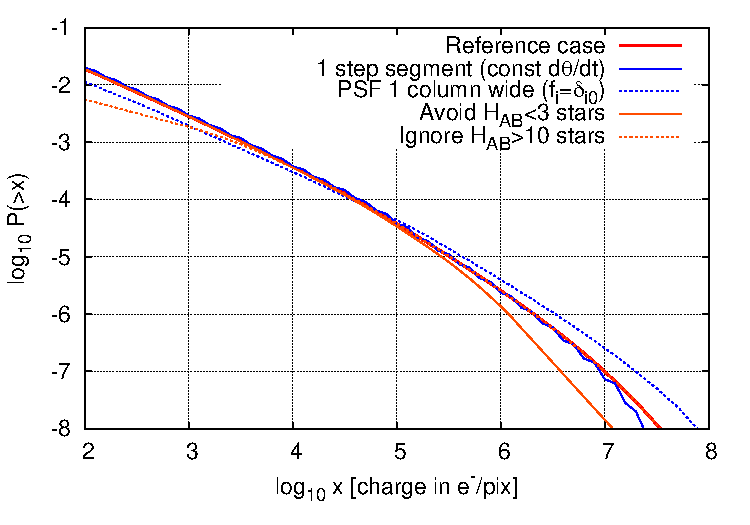
\includegraphics[width=5in]{Plots/slew_compare.pdf}
\caption{\label{fig:slewcompare}Comparison of stimulus levels predicted
under different assumptions and approximations. The vertical axis
shows the log probability to exceed a given stimulus level during a
slew of 0.4 degrees (a step along the short axis of the field,
executed frequently during the HLS). The thick red line indicates
reference assumptions. The solid blue line treats the slews as being
at constant $\dot\theta$. The dashed blue line approximates the PSF as
1 column wide (all the flux from the star is concentrated in the
central column). The orange lines show what happens if bright ($H_{\rm
AB}<3$) or faint ($H_{\rm AB}>10$) stars are excluded from the model.}
\end{figure}

\begin{figure}
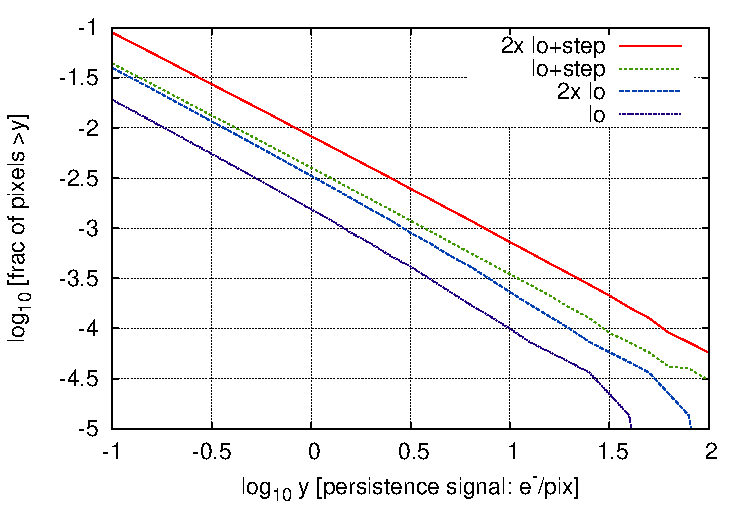
\includegraphics[width=5in]{Plots/sp_cdf.pdf}
\caption{\label{fig:sp_cdf}The cumulative distribution function of slew-induced persistence in the HLS imaging survey, $P(>y)$.
The persistence signal $y$ is estimated in electrons per pixel; the decaying persistence curve is integrated over a 160 s. Several persistence models are shown, including the ``lo'' case (typical of the development detectors), and a ``lo+step'' case (including an order of magnitude step at saturation, as seen in portions of some detectors). This figure has not been updated yet to go from the 6-year to the 5-year observing plan, although we expect only minor differences.}
\end{figure}

After negotiating with the Project, we settled on a mitigation strategy for slew persistence that involved saving the spacecraft orientation information from the Attitude Control System (ACS), using this to predict the locations of persistence from bright star streaks, and masking $\pm2\sigma$ on either side of these streaks. Unmasked streaks are simply accepted as part of the systematic error budget. Their impact on shape measurement is based on an analytic result derived by our SIT and tested against Monte Carlo simulations:
\begin{equation}
\Delta \gamma_1 + i\Delta \gamma_2 = \frac{M\Omega_{\rm
max}\sigma_{\rm n}^2 R^4}{2F^2N_{\rm ind}\,{\rm Res}} f_{\rm scale}
f_{\rm aniso},
\label{eq:dg}
\end{equation}
where $\Delta\gamma_{1,2}$ are the two components of spurious shear; $M$ is a margin factor; $\Omega_{\rm max} = 421.3$; $\sigma_{\rm n}^2$ is the variance of the persistence image; $R$ is the radius of the galaxy in pixels; $F$ is the signal from the galaxy in electrons per exposure; $N_{\rm ind}$ is the number of {\em independent} exposures of the galaxy\footnote{This may be less than the total number of exposures of the galaxy, since slew persistence from successive exposures will be correlated.}; Res is the galaxy resolution factor \cite{bej02}; $f_{\rm scale}$ and $f_{\rm aniso}$ are factors $\le 1$ describing the scale dependence and anisotropy of the persistence power spectrum (defined to be 1 in the worst case).

The results of this study -- shown in Figure~\ref{fig:slew_results_oct16} -- are promising, given the top-level systematic shear budget of $2.7\times 10^{-4}$ and that the modern detectors typically show ``lo'' or (in some regions) ``lo+step''-like behavior, rather than the much larger persistence characteristic of the WFC3-IR model (third column). The masking algorithm will continue to be revisited as part of the mission optimization. However, the small number of masked pixels led the FSWG to conclude that a dark shutter that operated during every slew was not required for the WFIRST HLS.

\begin{figure}
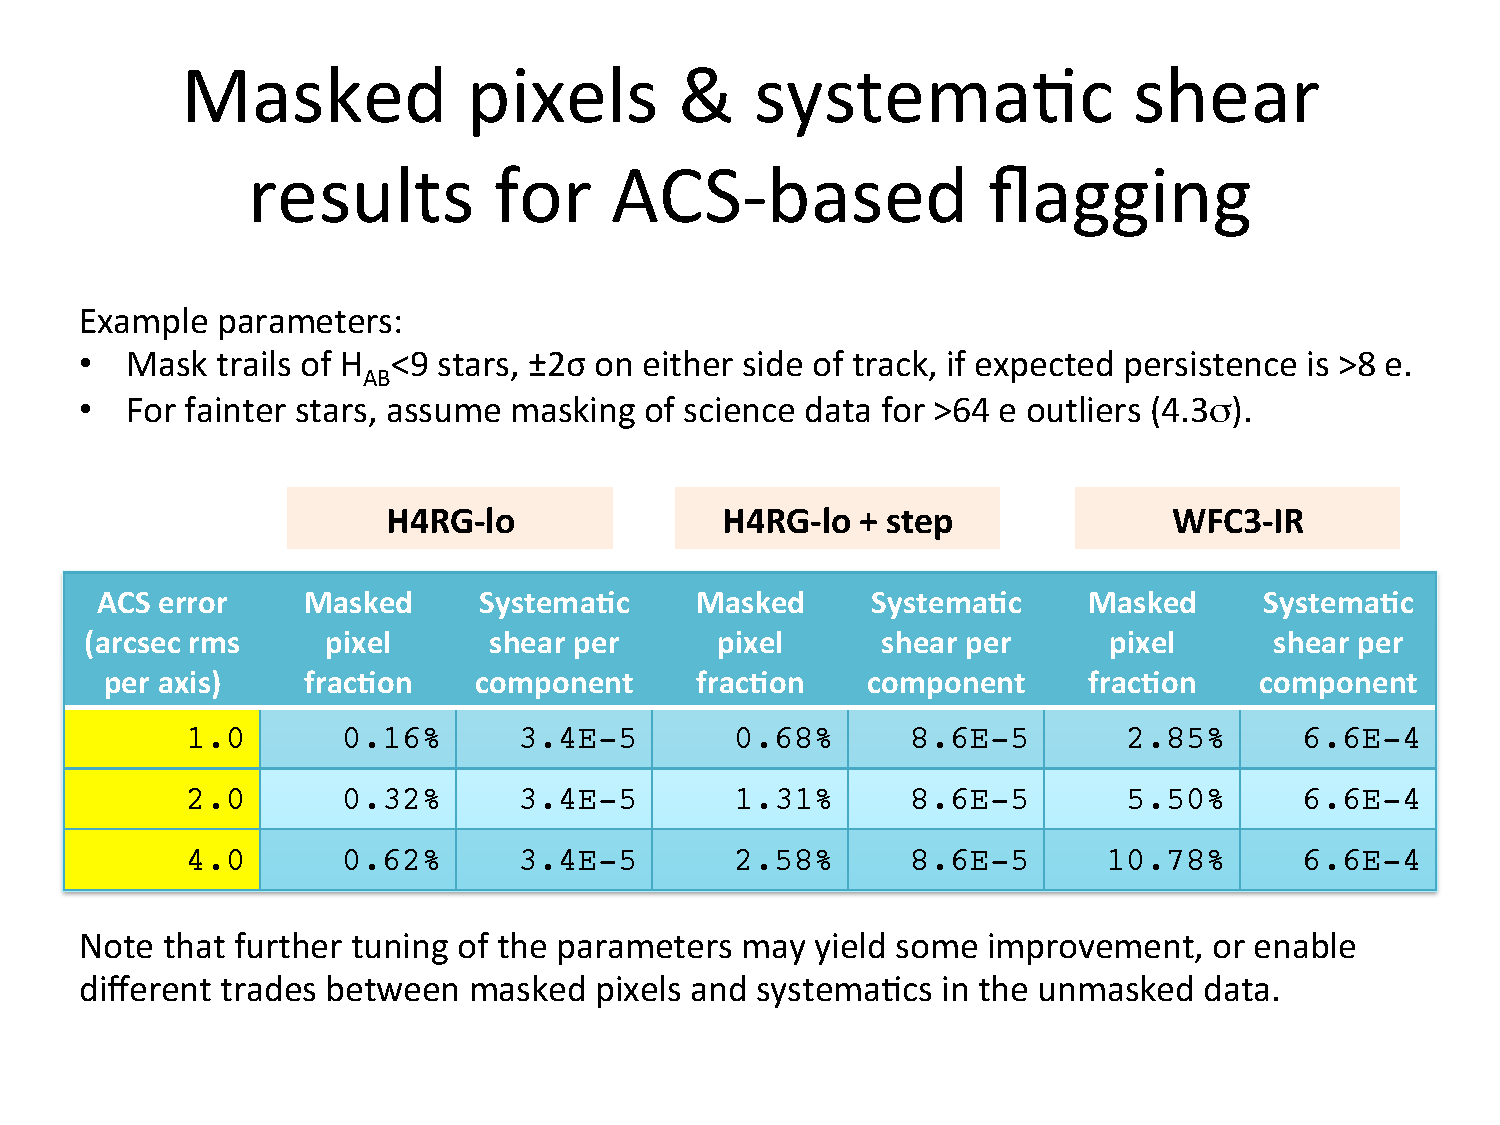
\includegraphics[width=5in]{Plots/slew_results_oct16.pdf}
\caption{\label{fig:slew_results_oct16}The outcome of the October 2016 slew persistence study. This shows the masked pixel fraction and the predicted systematic shear due to unmasked streaks as a function of both the persistence model and the accuracy of pointing information.}
\end{figure}

We carried out a related study, also using Eq.~(\ref{eq:dg}) and related machinery, to assess how well we need to know the dark current for WFIRST. Dark current measurements without a dark filter are possible, e.g.\ via median algorithms that combine many exposures from a survey, but are subject to: (i) a degeneracy in which the ``true'' sky brightness is unknown and hence the zero level of the dark current cannot be established, and (ii) possible correlated errors from imprinted celestial sources. The requirements, as derived in the appendix to the calibration plan, are:
\begin{list}{$\bullet$}{}
\item The error in the dark current + bias determination in a 140 s
HLS imaging exposure shall be no more than $0.0096f_{\rm corr}^{-1/2}$
e/p/s (uncorrelated part) or $0.0017 f_{\rm corr}^{-1/2}$ e/p/s
(imprinted celestial sources).
\item The error in the dark current + bias determination in a 297 s
HLS spectroscopy exposure shall be no more than $0.0059 f_{\rm
corr}^{-1/2}$ e/p/s (uncorrelated part) or $0.00072 f_{\rm
corr}^{-1/2}$ e/p/s (imprinted celestial sources).
\end{list}
Here ``$f_{\rm corr}$'' denotes the factor by which we plan to correct biases induced by errors in the dark current map (we normally choose $f_{\rm corr}=1$ to be conservative). The requirements are traceable to additive shear biases from non-circular imprinted celestial sources; multiplicative shear biases as the noise in the dark current map results in e.g.\ galaxy centroids getting ``pulled'' toward pixels whose measured dark current fluctuates below the true dark current of that pixel; and Eddington-like biases for sources detected in the GRS. While the semi-analytic estimates in the calibration plan based on source counts suggest that the HLS imaging requirement can be met without a dark filter, our SIT and the Calibration Working Group had concerns about possible degeneracies in the self-calibration procedure that can only be addressed by a detailed simulation. Moreover, the approach requires empty space in the images, which we will not have in the case of grism spectroscopy. As the imaging exposures are shorter than the spectroscopy exposures, this would require dedicated long imaging exposures (of HLS spectroscopy exposure length) just for the purpose of self-calibrating the dark. Due to sky Poisson noise, we would need many of these images -- our Feburary 2017 estimate was for $N=73$ exposures, which, if done every week, would consume 4\%\ of the wall clock time. In light of these and other issues, the Calibration Working Group recommended that WFIRST maintain the dark filter.

\subsubsection{Calibration Plan}
\label{sec:calibration_plan}
Our SIT has contributed extensively to the WFIRST WFI Calibration Plan. This includes extensive quantitative analysis of proposed calibration techniques, as detailed in the appendix to the plan. Some highlights follow.

The requirement on knowledge of the dark current and the calibration approaches are fully defined, based on analysis done during the dark filter trade (October 2016 -- February 2017).

Weak lensing was found to place demanding requirements on measurement of the count rate-dependent non-linearity (CRNL). The weak lensing program is sensitive to CRNL because it enhances the bright center of a PSF star relative to its wings, thereby making the star appear slightly smaller, but does not have a similar effect on the faint galaxies used for shape measurement. The PSF second moment is biased by a factor of $1-\alpha$ (where $\alpha$ is the CRNL exponent), and has a top-line systematic error budget of $7.2\times 10^{-4}$. This means that if $\alpha$ is measured to $\pm 3\times 10^{-4}$ (the requirement from the supernova SITs), then CRNL consumes 17\%\ of the PSF size error budget, in an RSS sense. Given that CRNL is a pernicious bias for two of the dark energy probes, we recommended a multi-faceted approach to CRNL calibration, including a lamp-on/lamp-off capability for WFIRST (this was not available on WFC3-IR).

Our team has revisited the wavefront stability requirements for weak lensing, using a set of codes and scripts on the team's GitHub site. This begins with a Fisher matrix analysis of the uncertainties in the shear power spectrum, and our top-line requirement that the systematic errors be equivalent to the statistical errors even if the survey is extended to 10,000 deg$^2$ (i.e.\ in an RSS sense, the systematic errors should be 20\%\ of the statistical errors in the nominal 2,000 deg$^2$ survey). Requirements are assessed using the significance, defined by
\begin{equation}
Z = \sqrt{\Delta{\bf C}\cdot{\bf\Sigma}^{-1}\Delta{\bf C}},
\label{eq:alpha}
\end{equation}
which is the number of sigmas at which one could distinguish the correct power spectrum from the power spectrum containing a systematic error. We built sub-allocations for multiplicative (shear calibration) errors, and for additive (spurious shear) errors in each angular bin. An early discovery was that this process depends on the redshift dependence of the shear error: some redshift dependences are ``worse'' than others by the $Z$-metric. The worst possibility is {\em not} for the error to be redshift-independent, but rather for it to change sign, as this can mimic a change in redshift evolution of the growth of structure.

In our current formalism, for each angular template, we introduce a limiting amplitude $A_0^{\rm flat}(\alpha)$, defined to be the RMS spurious shear per component $A_0$ at which we would saturate the requirement on $Z(\alpha)$ for angular bin $\alpha$ in the case of a redshift-independent systematic $w_i=1\,\forall i$ (here $\alpha$ denotes an angular bin and $i$ a redshift bin). That is, if the additive systematics did not depend on redshift, we could tolerate a total additive systematic shear of $A_0^{\rm flat}$ (RMS per component) in band $\alpha$. We also introduce a scaling factor $S[{\bf w},\alpha]$ for a systematic error
\begin{equation}
S[{\bf w},\alpha] = \frac{Z(\alpha) \,{\rm for\,this\,}w_i}{Z(\alpha)\,{\rm for\,all\,}w_i=1}
\end{equation}
that depends on the redshift dependence $w_i$. An additive systematic error that is independent of redshift will have $S=1$. A systematic that is ``made worse'' by its redshift dependence will have $S>1$, and a systematic that is ``made less serious'' by its redshift dependence will have $S<1$. The requirement that the (linear) sum of $Z$s not exceed $Z(\alpha)$ thus translates into
\begin{equation}
\sum_{\rm systematics} [A(\alpha)]^2\times S[{\bf w},\alpha] \le [A_0^{\rm flat}(\alpha)]^2,
\label{eq:A-S-sum}
\end{equation}
where $A(\alpha)$ is the RMS additive shear per component due to that systematic. We take the ``reference'' additive shear to be the additive shear in the most contaminated redshift slice; in this case, $w_i=1$ for that slice, and $|w_i|\le 1$ for the others. Under such
circumstances, we can determine a {\em worst-case scaling factor} $S_{\rm max,\pm}(\alpha)$, which is the largest value of $S[{\bf
w},\alpha]$ for any weights satisfying the above inequality. We may also determine a worst-case scaling factor $S_{\rm max,+}(\alpha)$
conditioned on $0\le w_i\le 1$, i.e.\ for sources of additive shear that have the same sign in all redshift bins. In most cases, however, something is known about the redshift dependence of the systematic error (e.g.\ for PSF errors the error scales with the size of the galaxy, and hence has a redshift dependence tied to the measured redshift evolution of galaxy sizes). In these cases, we use the correct redshift weighting factor $S$. This approach has been critical in order to set stability requirements that are consistent with the Project's integrated modeling results.

We have begun incorporating the HLS observing strategy (\S\ref{sec:operation}) in studies of self-calibration of time-dependent drifts in the response of the system (i.e.\ time dependence of the conversion from $\mu$Jy on the sky to DN/s in the digitized detector system outputs). This model is in a state of flux as we add parameters to it, but here we show a current snapshot allowing for time-dependent drifts of the response of each of the 18 SCAs making up the focal plane, with time dependence parameterized in calibration periods of $\Delta t$ (assessed down to a period of 3 hours) each. Both individual-SCA drifts and common-mode drifts are allowed, with an assumed intrinsic variation (calibration prior) of 1\%\ RMS drift in each $e$-fold of timescales. A network of randomly distributed stars with a density of 500 stars/deg$^2$ and $S/N=50$ was assumed; in self-calibration, the magnitudes of these stars are {\em not} known a priori, but are assumed to be stable across multiple repeated observations of the same field. These are preliminary parameters being used to test our tools and are not currently held as requirements. The stellar density model is very conservative since the Trilegal model predicts star counts of 572, 803, 990, and 1137 stars/deg$^2$ at $H_{\rm AB}=18-19$, $19-20$, $20-21$, and $21-22$ at the SGP, and even an $H_{\rm AB}=22$ star will have $S/N>50$. The temporal stability of the system needs further study and will be varied as an input parameter in future versions of this model. The current model uses the April 19, 2017 update to the HLS observing strategy. The number of calibration parameters varies depending on the filter, since there are no parameters for periods of time when the instrument is not observing in that filter; the current version has 17262 parameters for the H band.

Despite the intrinsic stability assumed, in which each SCA can have its response fluctuate by 1.67\%\ RMS from one time interval to the next, the repeated observations do an excellent job of tracking these changes and reducing the posterior uncertainty. Even for $\Delta t = 0.125\,$days$=3\,$hours, the posterior calibration errors are at the level of 0.14--0.17\%\ RMS (here ``RMS'' is weighted by number of observations), depending on the filter.  An example of the model output (predicted uncertainties in the calibration parameters for each SCA at each epoch) is shown in Figure~\ref{fig:hcalfig}. It must be remembered that this analysis is overly simplistic in some ways -- particularly that we have not yet allowed for shorter-timescale variations (i.e.\ on timescales $<\Delta t$), nor have we allowed for separate gain drifts among the different readout channels. These will have to be included in a future version of the model. On the other hand, the stellar density and $S/N$ assumptions were extremely conservative (e.g.\ the full range of stellar magnitudes 18--22 should have 7 times more stars than were assumed, even at the Galactic pole), so there is margin to absorb these additional degrees of freedom. The next iteration of the model for time-dependent calibration drifts will include additional parameters, as well as updated priors reflecting expected detector system stability rather than the place-holder requirements shown here.

\begin{figure}
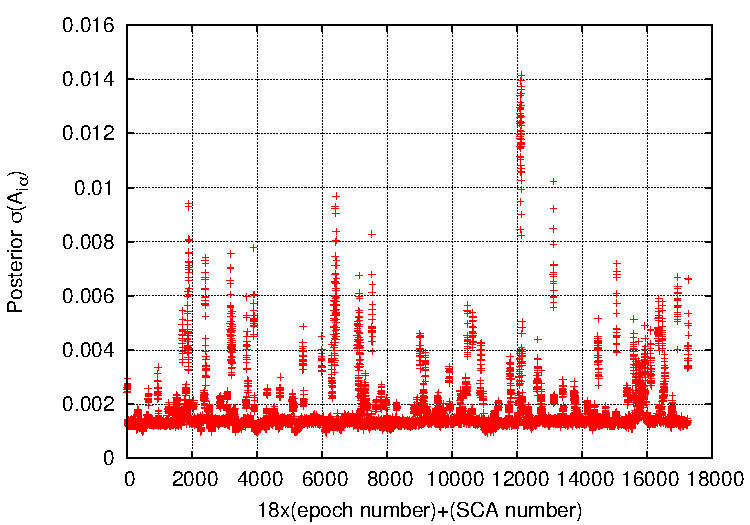
\includegraphics[width=4.5in]{Plots/hcalfig.pdf}
\caption{\label{fig:hcalfig}An example of the posterior calibration error from an HLS self-calibration calculation. The horizontal scale displays the time intervals (left-to-right in time order), with 18 points per time interval indicating the various SCAs. The vertical axis shows the standard deviation of the calibration solution for that SCA at that time, $\sigma(A_{i\alpha})$, relative to the survey mean. The figure shows the case of H band with $\Delta t = 0.125$ days. This example had 17262 calibration parameters. A few epochs, mostly containing only a few observations, are poorly constrained due to minimal overlap observations. It is subject to refinement and the input parameters of the model will be varied as we work toward requirements on the stability of the detector system.}
\end{figure}


\subsection{Identifying and Studying the Effect of Detector Imperfection (D3, D7)}
\label{sec:wl_detectors}
%================================================
\begin{summaryii}
  Since precision cosmology measurements depend sensitively on exquisite photometry; subtle effects that
  might not be noticeable in other areas of astrophysics can become important
  when trying to measure galaxy shapes to $<0.1$\%. Over the past year, we have
  studied novel possible systematic effects, implemented in an image
  simulation pipeline new and known effects and released it to the community. Our goal is to derive requirements for all these effects. Highlights include
  \begin{enumerate}
  \item The study of the effect of polarization-dependent quantum efficiency;
  \item The requirements on the interpixel capacitance;
  \item Detector characterization;
  \item Image simulation including detector imperfection and WFIRST scanning strategy to study their effect on shape measurement.
\end{enumerate}
In what follows, we provide some highlights from our detector characterization and simulation activities.
\end{summaryii}


\subsubsection{Polarization Effects}
During early 2017, work was carried out to assess the approximate level of an effect that could
cause weak lensing systematics, but that had never been previously considered by the weak lensing
community.  This effect is polarization-dependent quantum efficiency (due to e.g.\ different
reflectivity of various coatings for different polarizations of light).  Since the light from
edge-on disk galaxies typically has some low level polarization perpendicular to the disk, any
polarization-dependence of the QE could result in a preferential selection of such galaxies based on
their orientation in the focal plane.  This would violate the baseline assumption in a weak lensing
analysis, which is that all coherent galaxy alignments are due to gravitational lensing.

A student at CMU, Brent Tan, worked with Rachel Mandelbaum and Chris Hirata on a simple toy model
for this effect.  The toy model had two parameters: the fraction of the disk galaxy light that is
polarized, and the relative attenuation of that perpendicular polarization component (both numbers
in the range $[0,1]$).  For each point in that parameter space, the coherent shear due to selection
bias was calculated; see results in Figure~\ref{fig:polarization}.  Finally, the results were
modified to account for the fact that not all disk galaxies are viewed edge-on and that not all
galaxies are disks, giving a net coherent shear due to this selection bias of $\sim 3\times
10^{-4}$.  The results are still quite uncertain because our fiducial values for the disk
polarization fraction were based on observations of nearby galaxies, not $z\sim 1$ disks.  However,
this is large enough to be relevant for WFIRST, so this systematic needs to be evaluated more
carefully and requirements placed in future.  A publication on this topic will be prepared during
summer 2017.
\begin{figure}[t]
%\begin{center}
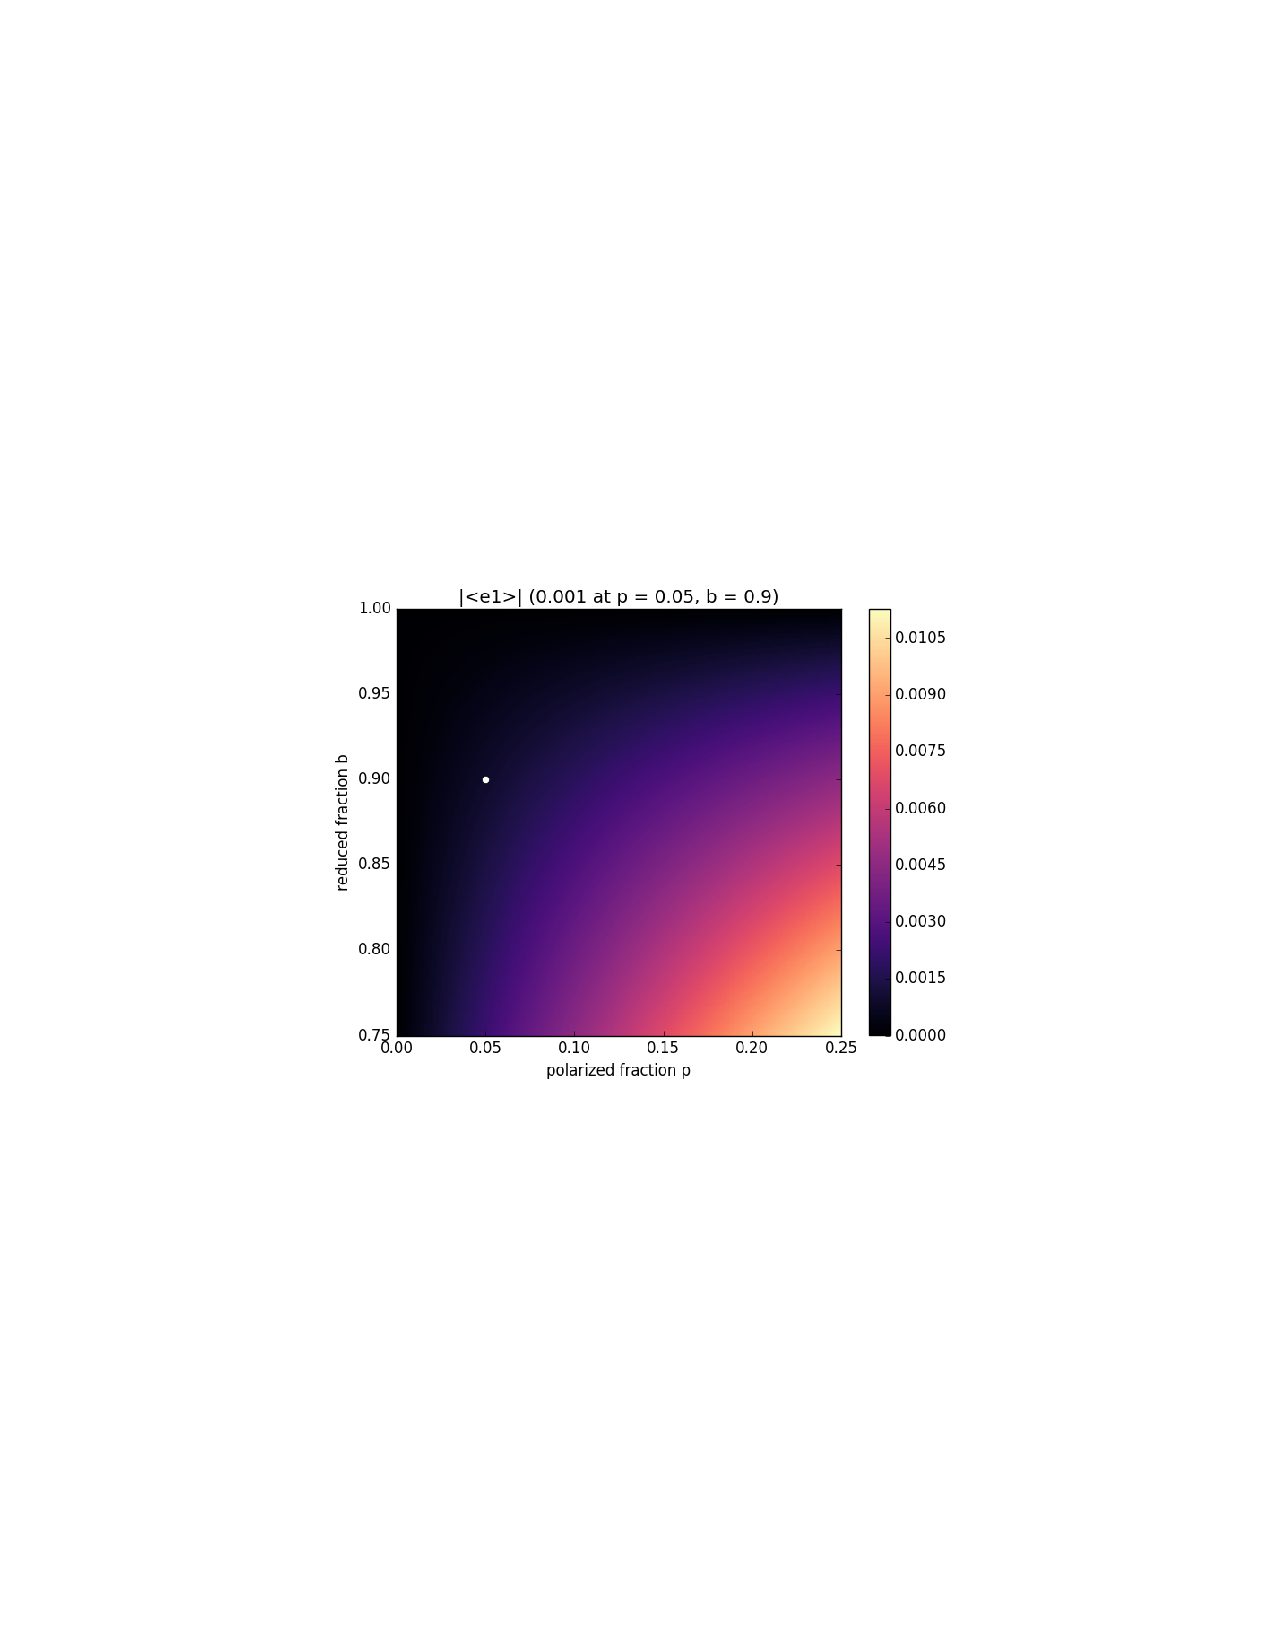
\includegraphics[width=0.66\textwidth]{Plots/polarization-selection.pdf}
%\end{center}
\caption{\label{fig:polarization}
The average shear due to weak lensing selection biases due to polarization-dependent quantum
efficiency, as a function of the fraction of polarized light from edge-on disks (horizontal axis)
and the fractional attenuation of the perpendicular polarization (vertical axis).  The dot at
$(0.05,0.9)$ is our fiducial point in parameter space, and has $\langle e\rangle \approx 0.001$.
}
\end{figure}

Another possible polarization-related systematic is a polarization-dependent PSF.  That will be the
subject of future work.

\subsubsection{Interpixel Capacitance Requirements}

The WFIRST detectors will suffer from electrical crosstalk between the pixels, unlike the optical
 detectors that are based on CCDs. This effect, known as the \emph{interpixel capacitance} (IPC),
 appears as a systematic effect in the weak lensing shear measurements and causes a
 bias in the measurements if not properly taken into account. The effect of IPC on the point-spread
 function (PSF) was already studied by members of our SIT in \cite{Kannawadi2016}, and requirements were placed
 on the level of uncertainty in the IPC based on how that uncertainty affects the PSF.

More recently, in late 2016, members of our SIT (Mandelbaum and student Kannawadi) carried out and
analyzed simulations to determine whether additional requirements on IPC are needed to ensure that
weak lensing shear estimation is not biased beyond our tolerances.  To calibrate the shear
multiplicative bias to an accuracy of $2\times 10^{-3}$, we find that the requirements on the IPC
placed by the PSF requirements are sufficient, so no new requirement is needed.  A paper on this
result is in preparation.


\begin{figure}[!t]
  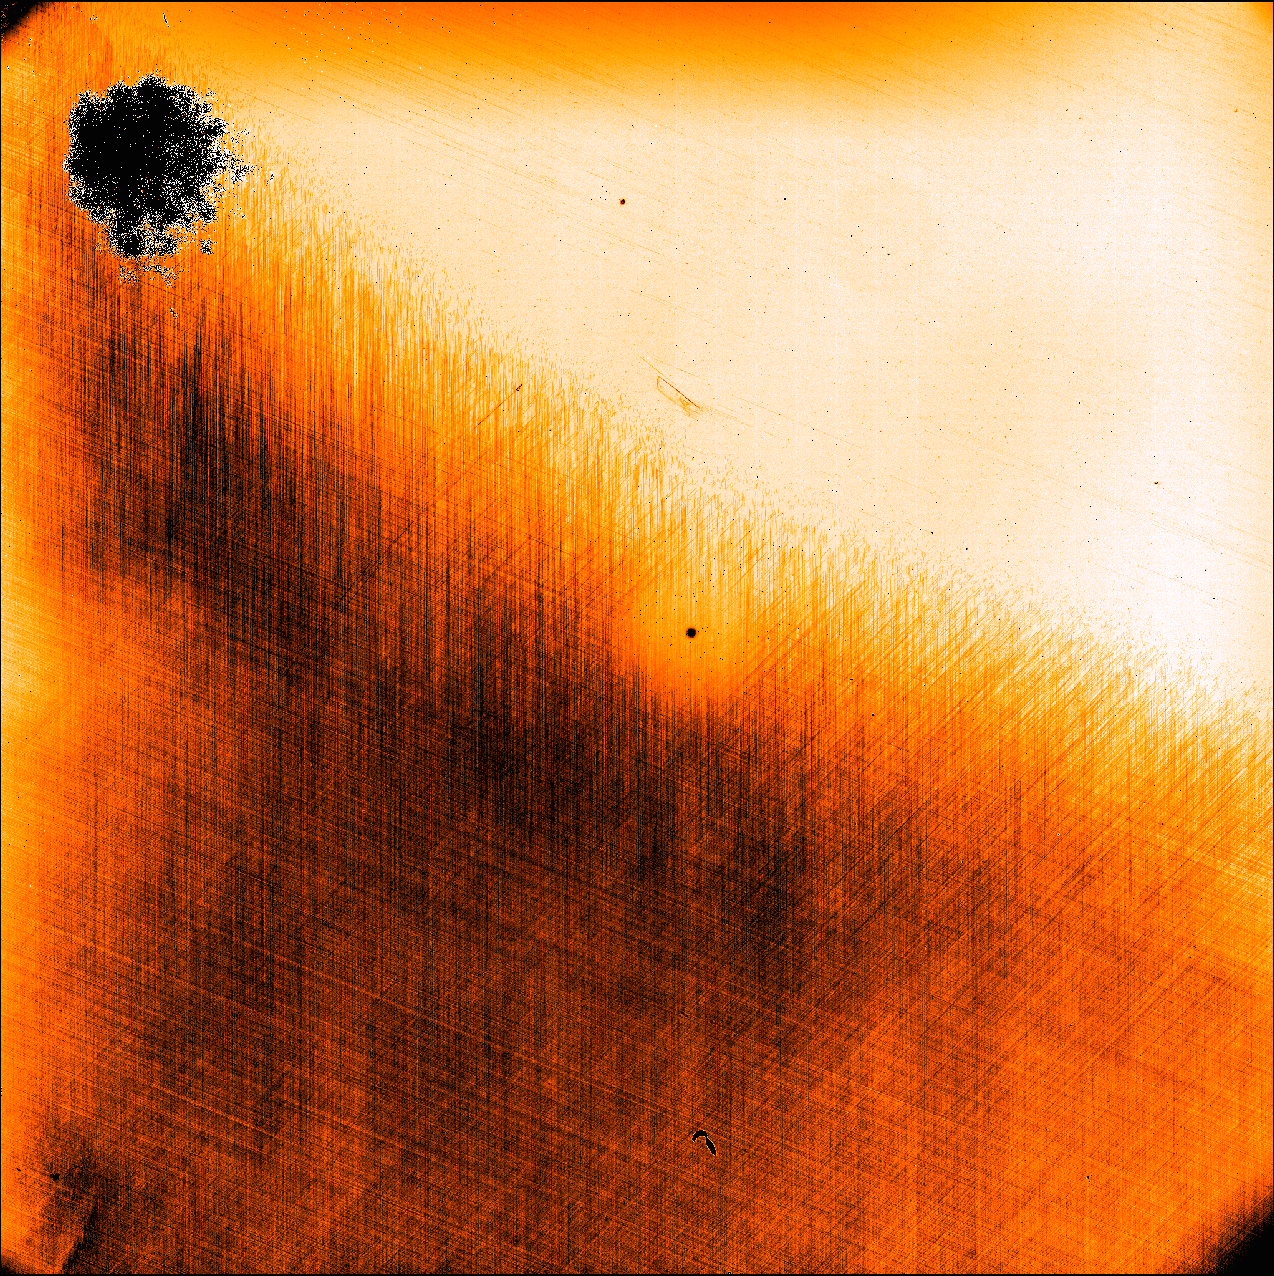
\includegraphics[width=0.55\textwidth]{Plots/Euclid_flat_crosshatch.png}
\caption{\label{fig:crosshatch}2048 x 2048 flat-field calibration image taken with a Euclid engineering grade H2RG detector (2.4 $\mu$m cutoff) under 1 $\mu$m illumination (scaled to enhance contrast).  Flight detectors resemble the upper right region (mean QE $\sim$ 1) but still contain traces of the ``crosshatch'' pattern visible in the lower left (mean QE $\sim$ 0.8).  Scanning a grid of undersampled point sources (f/11 aperture setting) in sub-pixel increments generated 1\% RMS photometric variations in the lower left region which were not removed by the flat-field calibration.  This result provides evidence that the pattern has intra-pixel structure that potentially biases the PSF if left uncalibrated.}
\end{figure}

\subsubsection{Laboratory Detector Characterization}

The WFIRST dark energy analyses will place enormous demands on our understanding
of the detectors. Some aspects of this problem can be anticipated in advance --
for example, we know that effects such as inter-pixel capacitance,
count-rate-dependent non-linearity  will need to be carefully
characterized, and we are working as part of the Calibration Working Group to
build these measurements into the mission. However, with systematic error
budgets at the level of a few$\times 10^{-4}$, it is likely that WFIRST analyses
will turn up new effects that were not apparent in past missions. Therefore a
key task for our SIT is to analyze the data from development detectors and
identify these new effects early enough to inform the calibration plan.

\begin{figure}[!t]
  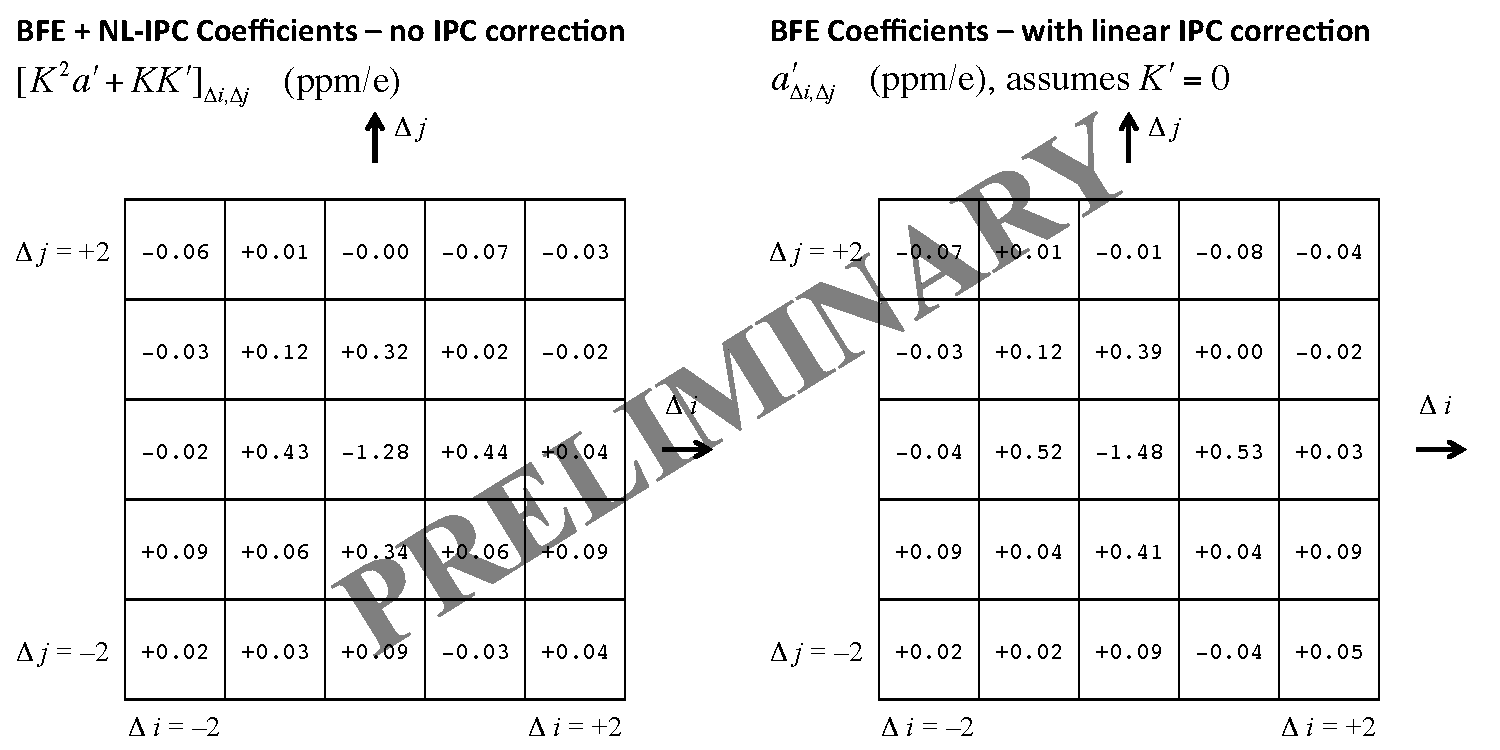
\includegraphics[width=6.2in]{Plots/kernel-17940B.pdf}
\caption{\label{fig:kernel}The BFE + NL-IPC coefficients $[K^2a'+KK']_{\Delta
i,\Delta j}$ (left panel) and IPC-corrected coefficients $a'_{\Delta i,\Delta
j}$ (right panel), for H4RG-17940. Note that the IPC-corrected coefficents
assume that the IPC is linear, i.e.\ the non-overlapping correlations are
ascribable entirely to the BFE and not NL-IPC. The $1\sigma$ uncertainty in each
pixel is 0.07 ppm/e.}
\end{figure}

In ground-based weak lensing projects using thick CCDs (e.g.\ DES), one of the
key detector issues has been the {\em brighter-fatter effect} (BFE). This is an
electrostatic effect in which as a pixel fills up with collected charge, it
changes the electric field geometry and new charges generated are more likely to
be deflected into neighboring pixels. This has the effect of making bright stars
appear larger than faint stars, as the repulsion effect is non-linear and
increases with signal level. The field geometry is very different in a NIR
detector, but a brighter-fatter effect is still possible.

We have searched for the brighter-fatter effect in the H4RG detector arrays
using the flat fields for two devices H4RG-17940 and H4RG-18237, provided to us
by the DCL. The BFE imprints a signature in the auto-correlation function of a
flat field; using the correlations in multiple non-destructive reads in a flat
field, one can separate linear IPC from the BFE. Preliminary brighter-fatter
effect results for H4RG-17940 are shown in Figure~\ref{fig:kernel}. The BFE
coefficients are $a'_{\Delta i,\Delta j}$, which is the fractional change in
effective area of pixel $(i,j)$ when an electron is placed in pixel $(i+\Delta
i, j+\Delta j)$; they have units of parts per million per electron (ppm/e). The
flat auto-correlations are sensitive to both the brighter-fatter effect and
non-linear inter-pixel capacitance (NL-IPC); we are currently working on
distinguishing the two effects.

We are also using data from studies of more mature H2RG detectors to inform our
calibration plan.  Although these will have important differences from the WFI
flight detectors, we expect that problematic effects discovered in H2RGs will
need to be characterized in H4RGs at some level.  For instance, collaborators
Shapiro and Huff (via the Precision Projector Laboratory at JPL) have
investigated a high-frequency pattern (dubbed the ``crosshatch'') apparent in
flat-field calibrations and believed to be related to the crystal structure of
HgCdTe (see Figure~\ref{fig:crosshatch}).  Using an engineering grade H2RG
provided by the Euclid mission, tests have shown that the crosshatch pattern
affects photometry even after flat-field calibrations are applied, implying that
it has sub-pixel structure that can bias PSF measurements.  Data was shared with
this SIT to investigate the dependence of the pattern on polarization and angle
of incidence.  The same H2RG detector is also being used to conduct a PSF-based
test of BFE to compare with our flat-field analysis.


\subsubsection{Simulating Detector Imperfection and Their Effect on WFIRST Shape Measurements}
\label{sec:hlis_image_sim}
Building on the existing GalSim framework and WFIRST module, Michael Troxel and Ami Choi (in collaboration with Hirata, Jarvis, Mandelbaum) are developing an image
simulation pipeline to assess the impact of various physical effects on the fidelity of the measured galaxy shapes.  The end product will provide realistic simulations containing all pertinent effects and conditions from the observational process specific to the WFIRST mission that may affect the quality of the lensing shear extracted
from the real WFIRST images.  These simulations will provide a foundation to characterize the relative impact of undesired effects and to validate the shear measurements themselves.  As the distribution and density of galaxies are realistically incorporated, the resulting multi-epoch images can also be used to test different dither strategies.  An intermediate level goal is to update the module with the most recent hardware and survey parameters describing the mission, to do some GalSim development to make the pipeline more efficient, and to estimate the relative impacts from detector effects such as the IPC described in earlier sections.

The pipeline is currently capable of simulating galaxies on individual postage stamps with a size and flux distribution drawn from the CANDELS catalog from Capak and Hemmati, a dither pattern from Hirata, realistic noise (see below), correct layout of SCAs, and options to dial a range of detector-level effects such as IPC, non-linearity, and reciprocity, among others.  The output simulated galaxies and truth tables are saved in Multi Epoch Data Structures (MEDS), which is a format commonly used in DES.  A publicly available shape measurement software, ngmix (\href{https://github.com/esheldon/ngmix/}), has been interfaced to measure shapes of the simulated galaxies.  Figure~\ref{fig:wl_imsim} illustrates a few of the effects in the context of a simulated bright, elliptical galaxy on a 32x32 pixel postage stamp.  The software is maintained in a repository available at \href{https://github.com/matroxel/wfirst_imsim} on GitHub.

The H4RG read noise model developed by \cite{Rauscher2015} can be straightforwardly incorporated into the simulations in order to study the effects of correlated noise on shape measurement.  Hirata has used simulations and a semi-analytic formalism to show that anisotropic noise induces additive ellipticity measurement errors, with the most damaging contributions coming from noise power at spatial wavelengths $\sim\pi R$ where $R$ is the observed scale radius of the galaxy or star.  With these tools, we will be able to derive requirements on detector noise and calibrate shape measurement pipelines to correct for remaining correlated noise.

\begin{figure*}[!t]
  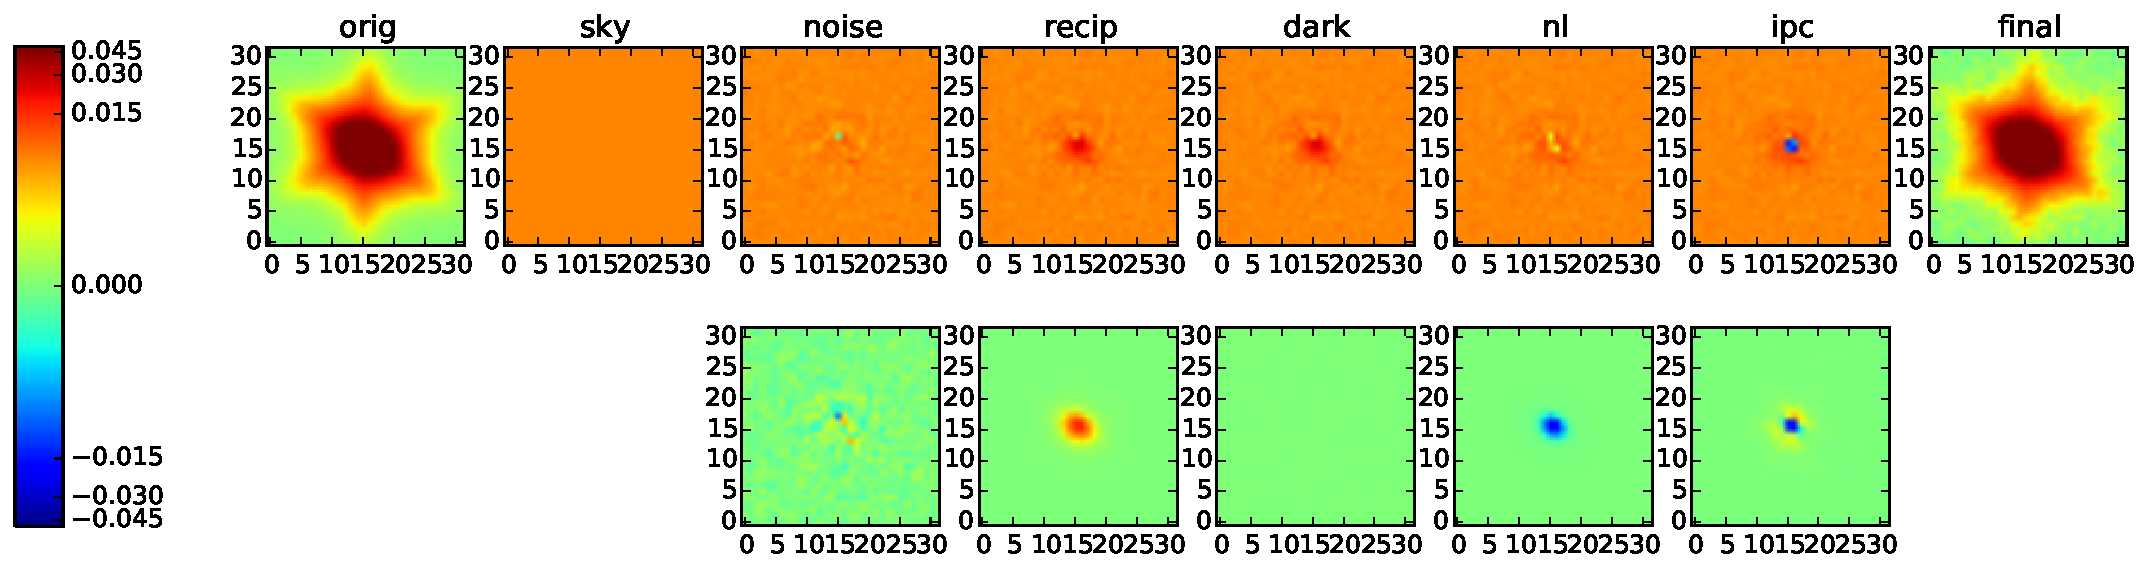
\includegraphics[width=0.9\textwidth]{Plots/wfirst_wl_imsim_example.pdf}
\caption{\label{fig:wl_imsim} An example of a simulated bright, elliptical galaxy produced by the image simulation pipeline.  The top row of subpanels begins with the original simulated bright elliptical galaxy (far left).  Each subpanel to the right of the original galaxy is a ``difference'' image that has the original galaxy subtracted off after the given effect (top label) has been applied.  These effects are: sky background, noise, reciprocity, dark current, nonlinearity, inter-pixel capacitance, respectively.  The bottom row of subpanels corresponds to the individual, isolated effects (top label).  The top, far right subpanel shows the final galaxy image after all effects have been applied.  The sub panels have been normalized by the maximum flux value of the original galaxy image, and the colors have been mapped to $\log_{10}$ values with a small range right around zero mapped to linear values as shown on a single colorbar corresponding to all of the subpanels.}
\end{figure*}

\begin{figure}
\centering
\begin{minipage}{.4\textwidth}
  \centering
  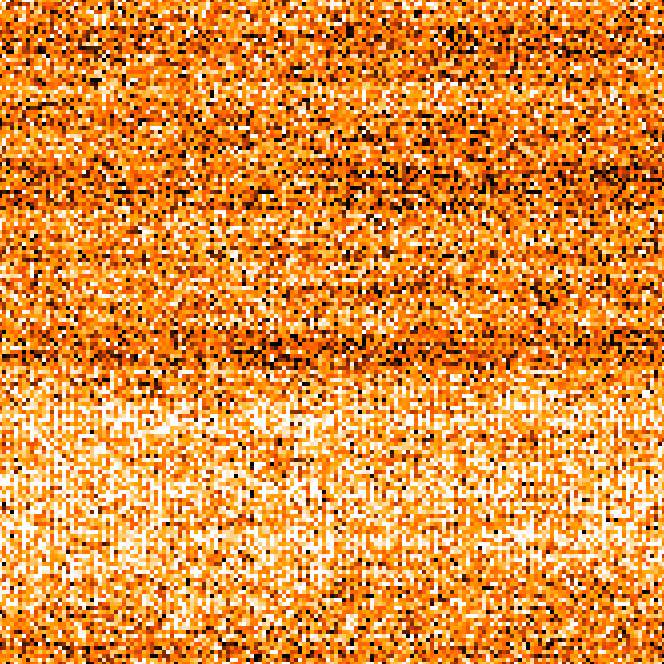
\includegraphics[width=.7\linewidth]{Plots/correlated_noise_sim.png}
\end{minipage}%
\begin{minipage}{.4\textwidth}
  \centering
  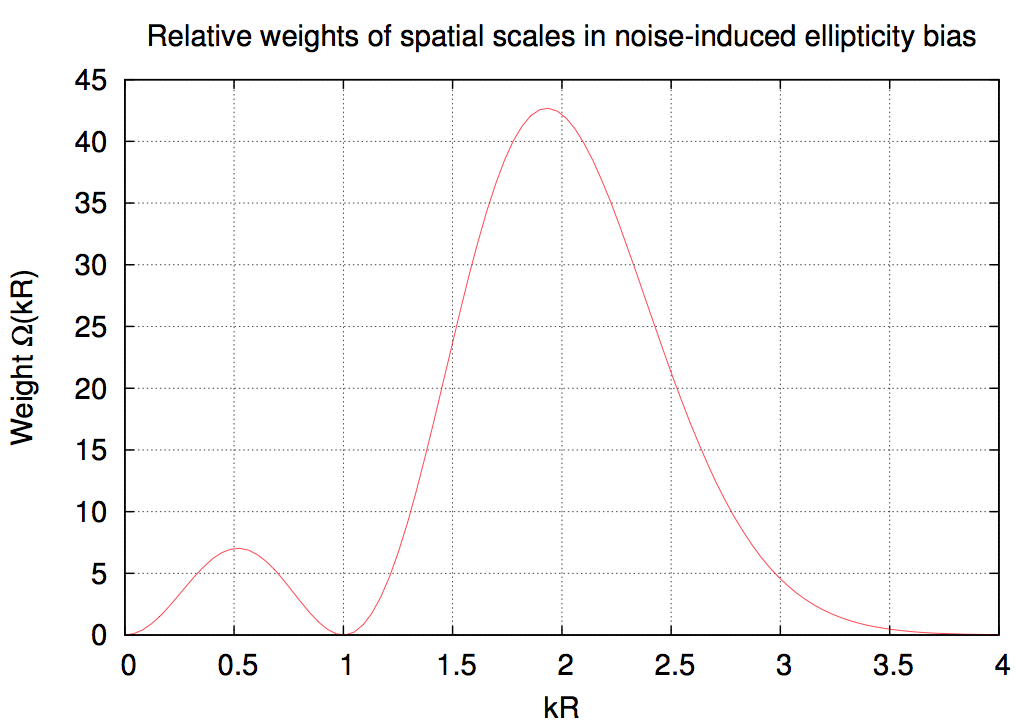
\includegraphics[width=1\linewidth]{Plots/correlated_noise_weight.png}
\end{minipage}
\caption{LEFT: Simulated noise in an H4RG subregion using the model of \cite{Rauscher2015}.  This image demonstrates the spatial effect of 1/f noise (horizonal bands) and alternating column noise (high frequency vertical striping).  RIGHT: Weight function showing the relative contribution of noise with spatial wavenumber $k$ to the ellipticity bias of a source with scale radius $R$.  For a given signal to noise level, the read noise shown would bias $e_1$ by different amounts for an undersampled PSF versus a larger galaxy.  This weight function assumes an adaptive moments shape measurement algorithm.}
\label{fig:correlated_noise}
\end{figure}

\subsection{Enabling Photometric Redshifts with WFIRST (D6, D11)}
\label{sec:wl_photoz}

\begin{summaryii}
Accurate photo-$z$s are crucial to all WFIRST probes of dark energy. In the
first year of SIT activity we have focused on developing accurate data-driven
simulations of the WFIRST lensing galaxy population and determining the
requirement on the spectroscopic samples needed to calibrate these photometric
redshifts. We proposed a plan to calibrate this sample and study the importance of the IFC. In the process, we generate new
data products that we released to other SITs and to the community.
\end{summaryii}

\begin{figure}
%\centering
 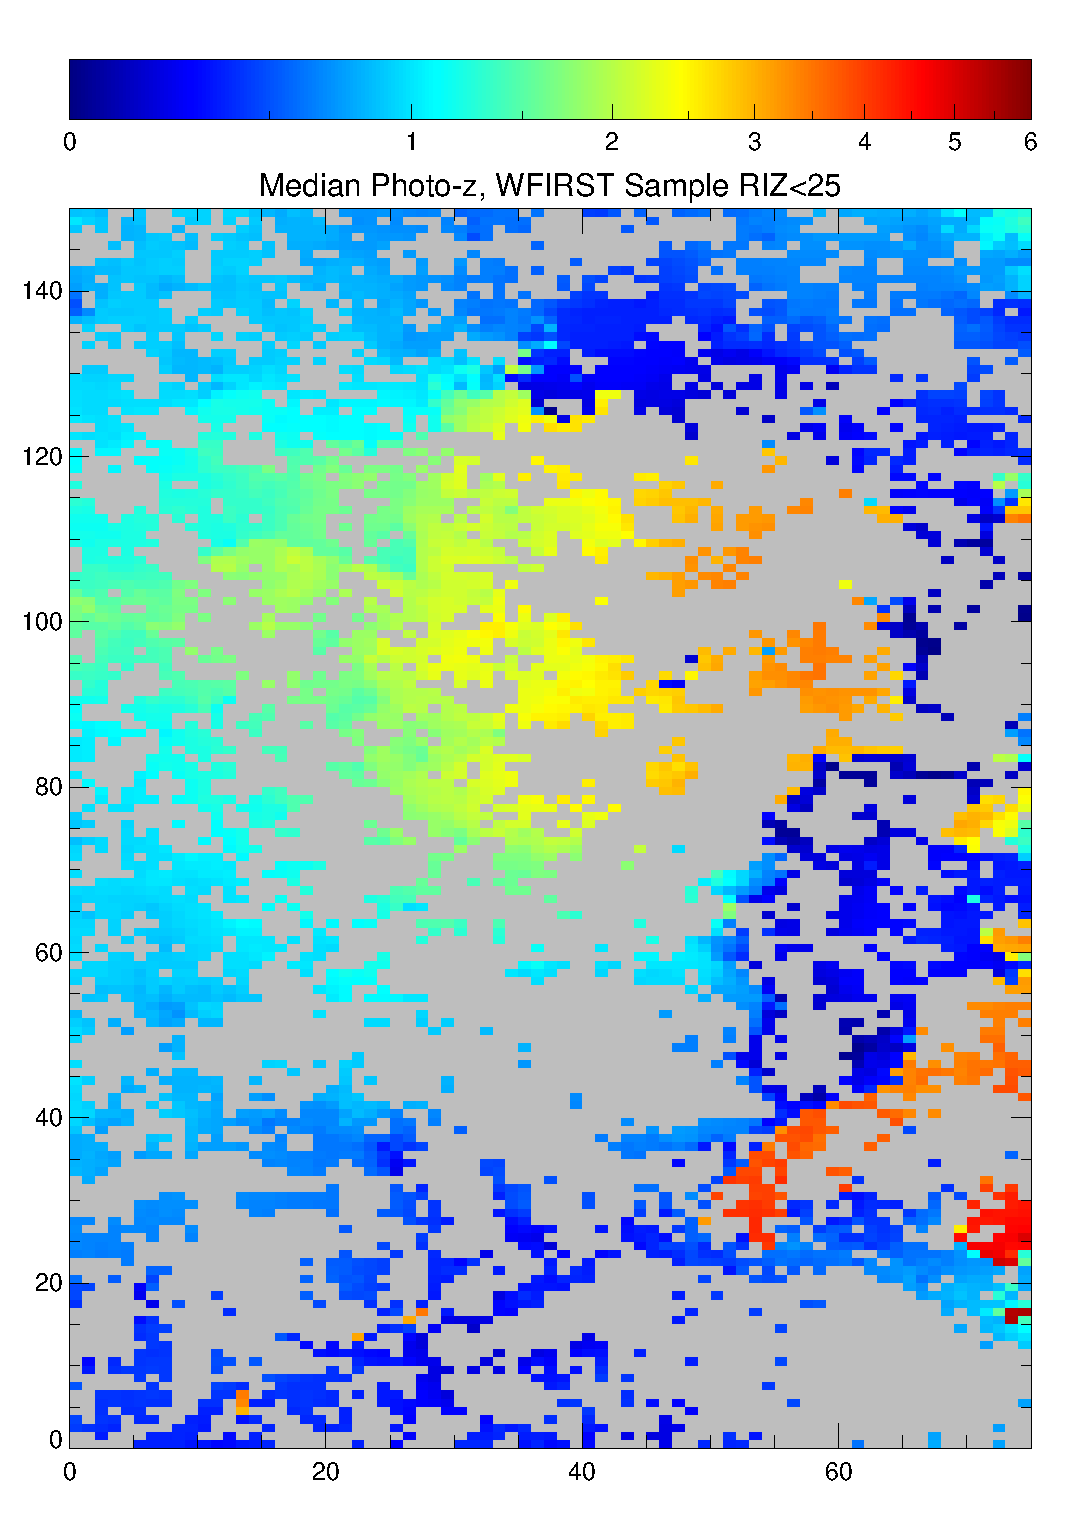
\includegraphics[width=0.45\textwidth] {./plots/wfirst_color_dist.eps}
\caption{A Self Organizing Map (SOM) \citep{Masters2015} of color space generated from $\sim6$ square degrees of data in the VVDS 2h, SXDS/UDS, COSMOS, and EGS survey areas colored by photometric redshift is shown.  Only regions occupied by the CANDELS survey are colored, with the remaining area grey.  CANDELS only covers 42\% of the color space, representing 49\% of the overall galaxy population.}
\label{fig:EuclidCandelsRep}
\end{figure}

\subsubsection{Generating Data-driven Simulations of WFIRST Galaxy Population}
\label{sec:candels}

The closest analogs to WFIRST data are the COSMOS and CANDELS HST surveys, however neither is fully analogous to
 WFIRST HLS data.  The COSMOS data cover 1.7 square degrees with HST-ACS (F814W)
 with ground based data analogous to LSST.  However, WFIRST analogous infrared
 data are not available over the majority of the field and extrapolations to the
 WFIRST lensing cuts from the F814W data over-estimate the number-density of
 sources usable for lensing.  In contrast, CANDELS has WFIRST analogous infrared
 data, but covers only 0.2 square degrees,which means it does not sample the
 full WFIRST galaxy population, and has very heterogeneous optical coverage.
 Specifically, a comparison between the CANDELS and COSMOS data to R,I,Z$<$25
 found that only 42\% of COSMOS galaxy colors (representing 49\% of the galaxy
 population) are present in CANDELS.  Figure~\ref{fig:EuclidCandelsRep} shows a
 Self Organizing Map (SOM) \citep{Masters2015} of the galaxy color space with
 regions where CANDELS galaxies fall marked.  The empty regions are shown in
 grey and correspond to cells with low galaxy density in COSMOS.  So these
 galaxies are simply less likely to be found in the relatively small area of
 CANDELS.

To overcome these limitations we have taken several approaches.  First, we have
collected a homogeneous 0.3-2.5$\mu$m data set over $\sim6$ square degrees in
the VVDS 2h, UDS/SXDS, COSMOS, and EGS fields.  These data are not as deep as
WFIRST, but are analogous to the LSST and Euclid data and allow us to estimate
the cosmic variance in galaxy population and estimate requirements on
spectroscopy.  These have been combined with the CANDELS catalogs which probe
WFIRST depth but are sample size and variance dominated.  We then adapted the
simulations described in \citet{stickley2016} developed for the SPHEREx mission
to assign a R$\sim$600 spectra to each object.  The CANDELS data are very
heterogeneous (see Table \ref{tbl:filters}), so we converted the various
photometric systems to a LSST+WFIRST system.  Figure~\ref{fig:filters} shows an
example of the LSST+WFIRST system along with the CANDELS filters on GOODS-S as
an example.  For the conversion we compared the converted photometry from other
bands to actual CFHT-LS $u^*$, $g^*$, $r^*$, $i^*$, $z^*$ and VISTA $Y$, $J$,
$H$, $K_s$ photometry in fields where they are available.   We found a simple
linear interpolation between filters in flux produced the best agreement.  Using
the \citet{stickley2016} or other template fits produced discretized value  in
the output fluxes which biased further analysis.

\begin{figure}
\centering
  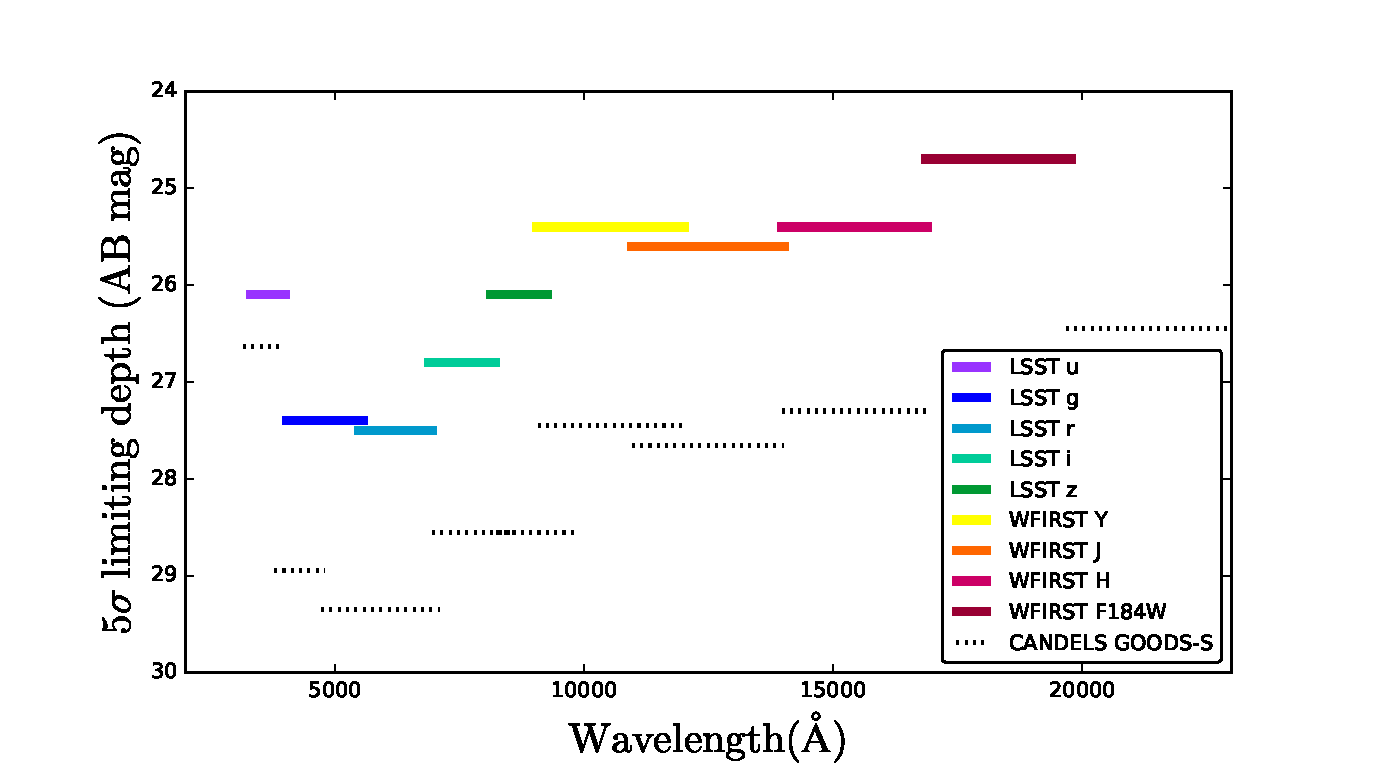
\includegraphics[trim=0cm 0cm 0cm 0cm, clip,width=0.50\textwidth] {./plots/filters.eps}
\caption{The 5$\sigma$ limiting AB magnitude of LSST and WFIRST filters plotted
as solid color lines and the 5$\sigma$ limiting AB magnitude of CANDELS GOODS-S
filters are plotted with dotted black lines (see Table \ref{tbl:filters} for
filter names).  Note the significant differences in the filter system which
necessitates conversion from one to the other.}
\label{fig:filters}
\end{figure}

The combination of these catalogs produces a reasonable estimate of the WFIRST
galaxy population for the purposes of assessing variance and the effects of
cuts.  However for some analysis a fully simulated catalog is required so that
the inputs are known perfectly.  To provide this we further adapted the methods
described in \citet{stickley2016} to produce simulated WFIRST+LSST photometry.
These three sets of simulated samples are being provided to other WFIRST SIT
teams for their analysis. Specifically we have been working with the Foley SNe focused SIT
team to simulate photo-$z$ performance for supernova cosmology.

%\begin{table}[h]
%\tabcolsep7.5pt
%\caption{Table caption}
%\label{tab1}
%\begin{center}
%\begin{tabular}{@{}l|c|c|c|c@{}}
%\hline

\begin{table}
\tabcolsep 2.8pt
\footnotesize
\caption{CANDELS filters in each field used to create the LSST+WFIRST catalog}
\begin{center}
\begin{tabular}{@{}*{15}{c}@{}}
\hline
\hline
\\
Field&&&&&&& Filters\footnote{\footnotesize Refer to CANDELS catalog papers for detailed description of observations in each filter, GOODs-S: \citealt{Guo2013}; GOODS-N: Barro et al. in prep; EGS: \citealt{Stefanon2017}; UDS:\citealt{Galametz2013}; COSMOS: \citealt{Nayyeri2017}}&&\\
\\
\hline
\\
GOODS-S& $\rm U_{VIMOS}$& $\rm F435W$& $\rm F606W$&$\rm F775W$ & $\rm F814W$ & $\rm F850lp$ & $\rm F098W$& $\rm F105W$ & $\rm F125W$ &$\rm F160W$&$\rm Ks_{HAWK-I}$\\
\\
GOODS-N&$\rm U_{KPNO}$& $\rm F435W$& $\rm F606W$&$\rm F775W$ & $\rm F814W$ & $\rm F850lp$ &$\rm F105W$ & $\rm F125W$ &$\rm F160W$& $\rm Ks_{CFHT}$\\
\\
EGS& $\rm U_{CFHT}$& $\rm g_{CFHT}$& $\rm F606W$ &$\rm r_{CFHT}$& $\rm i_{CFHT}$& $\rm F814W$ &$\rm z_{CFHT}$ & $\rm F125W$&$\rm F160W$&$\rm Ks_{CFHT}$\\
\\
UDS& $\rm U_{CFHT}$& $\rm B_{subaru}$&$\rm F606W$ &$\rm Rc_{subaru}$& $\rm i_{subaru}$&$\rm F814W$ &$\rm z_{subaru}$ & $\rm Y_{HAWK-I}$&$\rm F125W$&$\rm F160W$&$\rm Ks_{HAWK-I}$\\
\\
COSMOS&$\rm U_{CFHT}$& $\rm B_{subaru}$& $\rm F606W$&$\rm r_{subaru}$&$\rm i_{CFHT}$&$\rm F814W$ &$\rm z_{CFHT}$ & $\rm Y_{UVISTA}$&$\rm F125W$&$\rm F160W$& $\rm Ks_{UVISTA}$\\
\\
\hline
\end{tabular}
\end{center}
\label{tbl:filters}
\end{table}

\begin{figure}
\centering
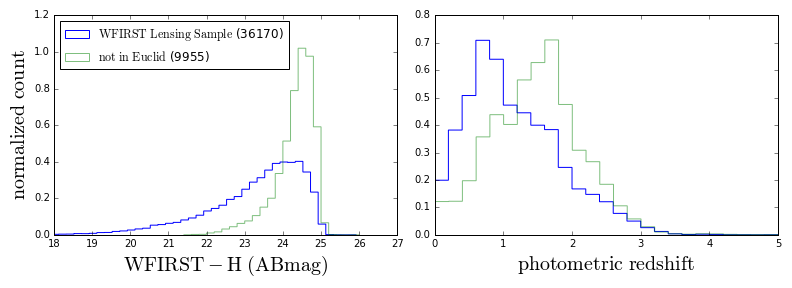
\includegraphics[trim=0cm 0cm 0cm 0cm, clip,width=0.95\textwidth] {./plots/histogram_wfirst_notEuclid.png}
\caption{{\bf Left:} A magnitude histogram of the WFIRST lensing sample split
into a C3R2 Euclid like lensing sample (blue, $RIZ<25$) and those only in WFIRST
(green).  Roughly 20\% of the WFIRST sample consists of galaxies fainter than
what C3R2 is calibrating for Euclid.  Note the Euclid lensing sample is cut at
$RIZ<24.5$, shallower than the proposed calibration \citep{Masters2015}.  {\bf
Right:} The redshift distribution of the C3R2-Euclid sample (blue) and the
WFIRST only sample (green) are shown normalized to an integral of 1. Even though
the WFIRST galaxies are fainter than the calibration limit they cover a redshift
range similar, just with with more galaxies at high-redshift.   }
\label{fig:EuclidVsWFIRST}
\end{figure}

\begin{figure}
\centering
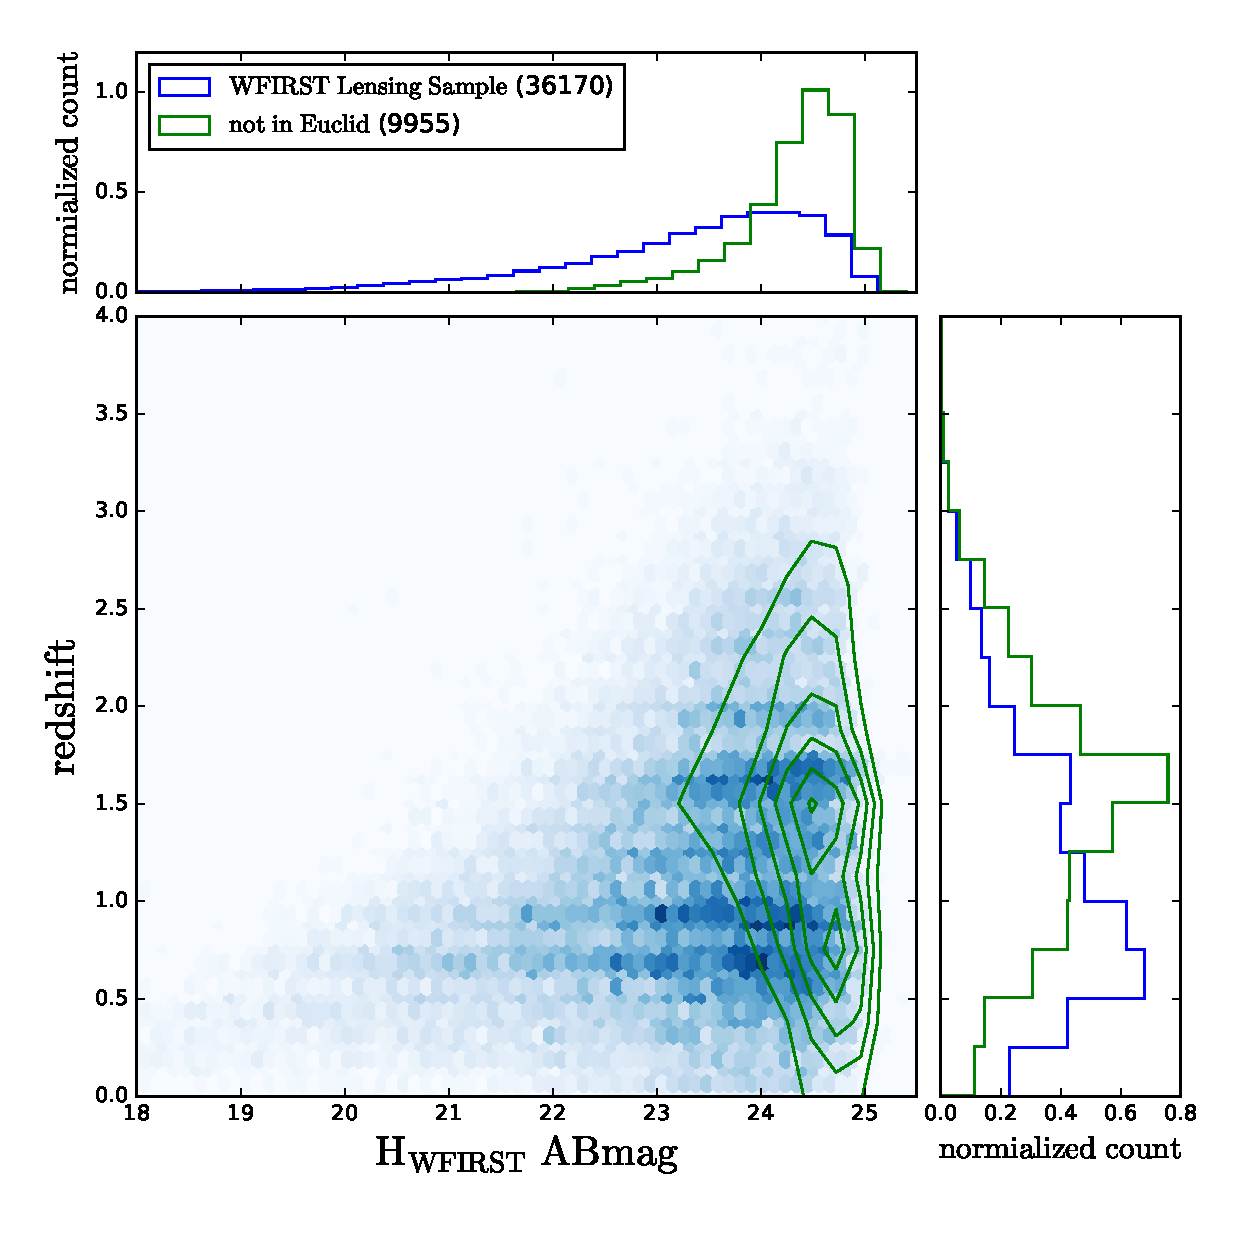
\includegraphics[trim=0cm 0cm 0cm 0cm, clip,width=0.75\textwidth] {./plots/redshift_magnitude.eps}
\caption{$H$ band magnitude vs redshift is plotted for the WFIRST lensing sample
shown in Figure \ref{fig:EuclidVsWFIRST} with shading indicating relative
density.  The WFIRST only sample shown as green contours and the histograms from
from Figure \ref{fig:EuclidVsWFIRST} are plotted on the axis.   }
\label{fig:EuclidVsWFIRST2}
\end{figure}

\subsubsection{Calibrating the Photometric Redshifts of WFIRST Weak Lensing Galaxy Population}

These simulations have been used for several analyses within our SIT.  Figure~\ref{fig:EuclidVsWFIRST} shows the relative differences in the magnitude and
redshift distribution of the total Euclid and WFIRST faint lensing samples.
WFIRST clearly adds fainter and higher-redshift systems to the weak lensing
sample.  However, Figure \ref{fig:WFIRSTSOM} shows a Self-Organizing-Map
analysis \citep{Masters2015} of the WFIRST lensing sample compared with the
Euclid sample. Even though WFIRST is significantly fainter than Euclid, 96\% of
galaxies fainter than the Euclid sample have color analogs at brighter
magnitudes.  The implication is that while WFIRST is seeing fainter galaxies
than Euclid, these galaxies are very similar to less numerous but brighter
systems seen by Euclid.

\begin{figure}
\centering
 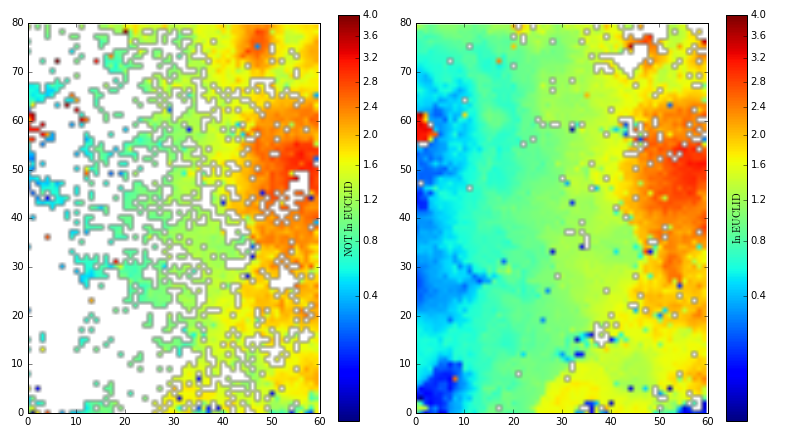
\includegraphics[trim=0cm 0cm 0cm 0cm, clip,width=0.98\textwidth] {./plots/SOM_WFIRST_EUCLID.png}
\caption{A Self Organizing Map (SOM) \citep{Masters2015} of the WFIRST color
space based on the CANDELS data cut to the WFIRST lensing sample color coded by
their median redshift.  The left panel shows SOM cells that contain galaxies too
faint to be in the C3R2 RIZ$<25$ Euclid like sample
\citep{Masters2015,Masters2017}.  The right panel shows SOM cells with galaxies
that are in the C3R2 sample.  $\sim96\%$ of the WFIRST color space is occupied
by galaxies in the C3R2 sample, however $\sim20\%$ of the WFIRST sample is
fainter than the C3R2 limit.  This means their calibration would have to be
verified to ensure no magnitude dependence on redshift. }
\label{fig:WFIRSTSOM}
\end{figure}

To determine how difficult it would be to obtain spectra for these faint systems
we conducted an analysis of the R$\sim$600 SEDs fit to the photometry.  Based on
the C3R2 survey spectra \citep{Masters2017} we developed a spectral simulator
which accurately re-produces ground based spectra for Keck DEIMOS, LRIS, and
MOSFIRE.  In addition to these instruments the simulated response of the
WFIRST-IFC was simulated.  Example simulated spectra based on the model fits
along with actual Keck spectra obtained for those sources are shown in Figure
\ref{fig:SpecSim}.

\begin{figure}
\centering
 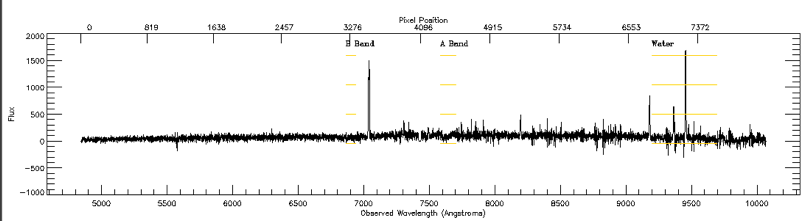
\includegraphics[trim=0cm 0cm 0cm 0cm, clip,width=0.45\textwidth] {./plots/realspec.png}\\
   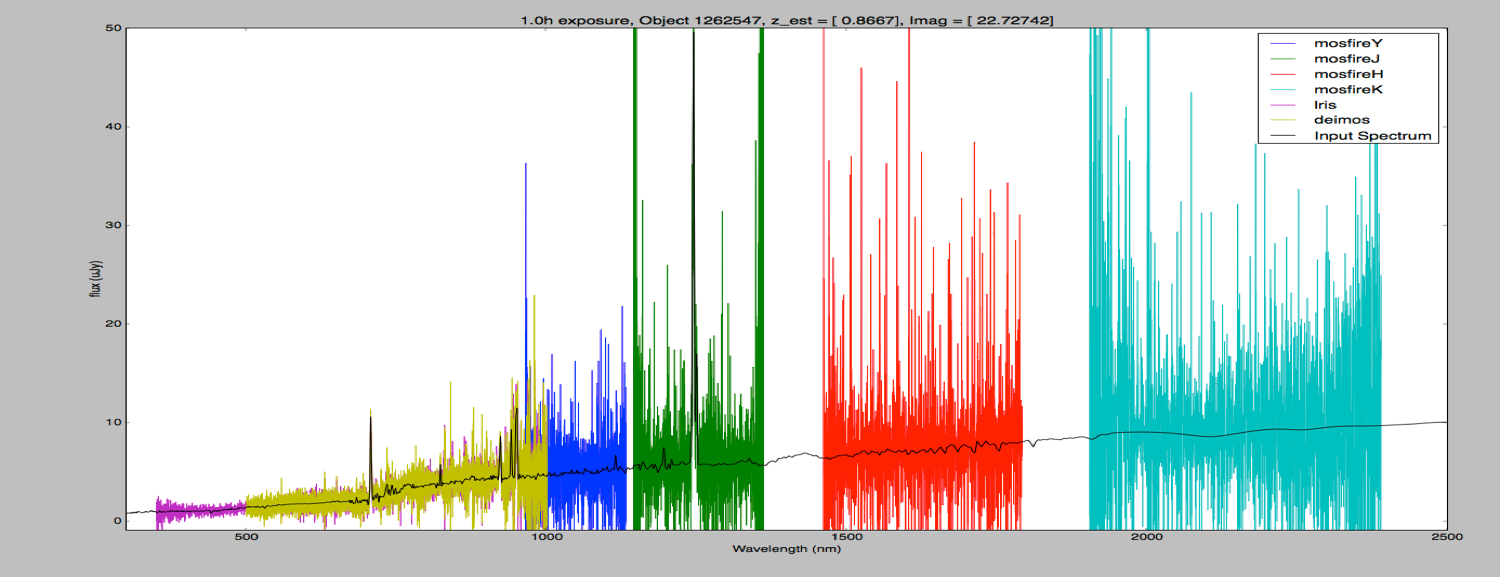
\includegraphics[trim=0cm 0cm 0cm 0cm, clip,width=0.45\textwidth] {./plots/simspec.png}

\caption{ A real (top) and simulated (bottom) spectra of a $I=22.7$ galaxy in the C3R2 sample.}
\label{fig:SpecSim}
\end{figure}

We found that indeed most of the faint WFIRST lensing galaxies were analogs of
brighter systems. This alleviates the need to obtain spectroscopic redshifts to
this population since the color-redshift relation will be known.  However, steps
must be taken to validate that the redshift distribution does not change at
fainter magnitudes in ways not apparent in the WIFRST+LSST colors.

The simplest method would be to extend a survey such as C3R2 \citep{Masters2017}
to fainter magnitudes. However, these faint galaxies are difficult to obtain
high-quality spectra for from the ground.  For the purposes of this analysis we
define high quality as an SNR$>$7 on two emission features or an SNR$\sim5$ on
an underlying continuum.  Based on this criteria, 20\% of the WFIRST color space
requires $>5$h spectra from Keck.  It is important to note this is in terms of
color space, and the exact number of spectra required to calibrate this color
space will require further analysis.   Of these, 1\% are sources that require
long ground exposures due to strong emission lines falling between ground based
observing windows and spectra could be obtained with the WFIRST grism.  A
further 15\% would have high-quality redshifts with WFIRST-IFC parallel
observations based on simulating the spectra and assessing the number of
features with SNR$>$7.  However, due to the low-resolution of the WFIRST-IFC
further analysis may be merited.   The remaining 4\% of galaxies could not be
calibrated by WFIRST or from the ground with 10m telescopes and would require
either ELTs or JWST.

\subsection{Cluster Cosmology with WFIRST}

\begin{summaryii}
Our work during the past year has focused on building machinery
for comprehensive cosmological forecasts for the WFIRST cluster
program that will include representations of the most significant
anticipated systematic effects.
\end{summaryii}

Cluster cosmology is generally considered to be less demanding in terms of
hardware requirements than cosmic shear, since the large galaxy over-densities
and shear signals are not as easily masked by subtle optical aberrations or
detector behaviors. Nevertheless, it may place new requirements on survey
footprint/operations (to ensure overlap with other data sets); pipeline behavior
in crowded fields (e.g., \cite{2015MNRAS.449.1259S}); and ancillary data
products and simulations to describe, e.g., changes in selection effects and
source redshift distributions in the presence of blending and magnification.

% As described in our proposal, we are treating the WFIRST cluster cosmology program as essentially a subset of weak lensing.
 Clusters can be identified
 using galaxy counts in WFIRST and external data, or from X-ray or
 Sunyaev-Zeldovich surveys.  WFIRST yields high-precision measurements of
 cluster weak lensing shear profiles, which can be combined with cluster
 abundances and cluster-galaxy cross-correlations to derive cosmological
 parameter constraints, most notably on the amplitude of matter clustering.

We have verified our ability to reproduce previous forecasts quantitatively with
new and independent code -- a non-trivial exercise that required resolving
ambiguities about halo mass definitions, source redshift distributions, and so
forth. We have extended the new code so that it can simultaneously model weak
lensing signals from small scales (the ``one-halo'' regime) out to large scales
described by linear theory. To achieve accurate results in the transition
between these regimes, we have developed a numerically calibrated prescription
for mass profiles in the ``splashback'' zone beyond the cluster virial radius.
These numerical calibrations are based on a suite of cosmological N-body
simulations that we are using to create full numerical ``emulators'' for
cluster-mass and cluster-galaxy cross-correlation functions, using parameterized
halo occupation distributions to relate galaxy populations to the underlying
dark halo population. We are exploring the degree to which cluster-galaxy
cross-correlations can sharpen cosmological constraints when combined with
cluster weak lensing; we anticipate including these cross-correlations in our
cosmological forecasts at a later time.

Our current focus is on incorporating a realistic description of photometric
redshift distributions and nuisance parameters that describe systematic
uncertainties in those distributions. Our hope is that the combination of cosmic
shear and cluster weak lensing measurements will prove much more robust to
photometric redshift uncertainties than either technique individually, because
the two methods have somewhat different dependence on source redshifts, and
because the redshifts of the clusters themselves are accurately known. We will
then turn to nuisance parameters that describe uncertainties in the clusters
themselves, e.g., contamination, incompleteness, mis-centering, and projection
biases in cluster selection.

Collaborator Anja von der Linden presented a technical overview of the WFIRST
cluster program at the January 2017 WFIRST Science meeting at the Center for
Computational Astrophysics, with an emphasis on the opportunities and
requirements for joint analyses with LSST and Sunyaev-Zeldovich surveys.
Collaborator Eduardo Rozo, together with Eli Rykoff, has been leading efforts in
cluster identification in the Dark Energy Survey (DES), building on their
earlier work with the Sloan Digital Sky Survey.  Rozo is also leading the
cluster cosmology analyses in the DES, with Year 1 DES results expected in a few
months. WFIRST cluster identification and analysis methods will build on the DES
techniques, and the lessons from applying these techniques to state-of-the-art
wide-field survey data will be invaluable for WFIRST planning.
